\documentclass{Nan_Thesis}
\usepackage{graphicx}
\usepackage{float}
\usepackage[hyphens]{url}
\usepackage[hidelinks]{hyperref}
\usepackage{booktabs}
\hypersetup{breaklinks=true} 
%\documentclass[nofigurelist, notablelist,proposal]{uofsthesis-cs}
% Documentation for the uofsthesis-cs class is given in uofsthesis-cs.dvi
% 
% It is recommended that you read the CGSR thesis preparation
% guidelines before proceeding.
% They can be found at http://www.usask.ca/cgsr/thesis/index.htm

%%%%%%%%%%%%%%%%%%%%%%%%%%%%%%%%%%%%%%%%%%%%%%%%%%%%%%%%%%%%%%%%%%%%%%%%%%%%%%
% FRONTMATTER - In this section, specify information to be used to
% typeset the thesis frontmatter.
%%%%%%%%%%%%%%%%%%%%%%%%%%%%%%%%%%%%%%%%%%%%%%%%%%%%%%%%%%%%%%%%%%%%%%%%%%%%%%

% THESIS TITLE
% Specify the title. Set the capitalization how you want it.
\title{Bluetooth Low Energy Based CoAP Communication in IoT \\ CoAPNonIP: An Architecture Grants CoAP in Wireless Personal Area Network} 
% AUTHOR'S NAME
% Your name goes here.
\author{NAN CHEN}

% DEGREE SOUGHT.  
% Use \MSc or \PhD here
\degree{\MSc}         

% EXPECTED CONVOCATION DATE
% Should be month/year, e.g. July 2004
\convocationdate{Month/Year}


% NAME OF ACADEMIC UNIT
%
% The following two commands allow you to specify the academic unit you belong to.
% This will appear on the title page as
% ``<academic unit> of <department>''.
% So if you are in the division of biomedical engineering you would need to do:
% \department{Biomedical Engineering}
% \academicunit{Division}
%
% The default is ``Department of Computer Science'' if these commands
% are not given.
%
% If you are in a discipline other than Computer Science, uncomment the following line and
% specify your discipline/department.  Default is 'Computer Science'.
% \department{If not Computer Science, put the name of your department here}

% If you are not in a department, but say, a division, uncomment the following line.
% \academicunit{Put the type of academic unit you belong to here, e.g. Division, College}


% PERMISSION TO USE ADDRESS
%
% If you are not in Compuer Science you will want to change the
% address on the Permission to Use page.  This is done using the
% \ptuaddress{}.  Example:
%
% \ptuaddress{Head of the Department of Computer Science\\
% 176 Thorvaldson Building\\
% 110 Science Place\\
% University of Saskatchewan\\
% Saskatoon, Saskatchewan\\
% Canada\\
% S7N 5C9
% }

% ABSTRACT
\abstract{
In recent years, the development of smart devices has led to the Internet of Things (IoT). In IoT, the Constrained Application Protocol (CoAP) is a well-known protocol used in constrained networks. CoAP aims to work in IP-based networks. However, there are many constrained devices using different scenarios to transfer data. For example, Bluetooth Low Energy (BLE) devices use the Media Access Control (MAC) address as an identifier and use Generic Attribute Profile (GATT) to transfer data. Therefore, how to overcome those barriers is an important topic. There are several approaches to overcome those barriers. For example, a new hardware component can be added to make those devices support TCP/IP protocol stacks, then CoAP can easily be implemented in those devices. On the other hand, an application layer architecture can be added upon existing communication technologies to support CoAP. Considering to minimize the changes of underlying communication infrastructure, the second approach can achieve the goal with less effort.

This thesis proposes an architecture that apply CoAP to different Non-IP based communication technologies. Meanwhile, Bluetooth Low Energy is used to explore how to overcome limitations of underlying technology. By adopting the proposed architecture, existing devices can participate in the IoT through CoAP without extra hardware upgrade or hardware modification. Although my experiment shows the current implementation of the proposed architecture has relatively low data rate, the problem can be solved by changing factory settings of the BLE devices. Compared with hardware solution, the proposed architecture takes less effort to support different underlying technologies and platforms.
}

% THESIS ACKNOWLEDGEMENTS -- This can be free-form.
\acknowledgements{
I would like to express my very great appreciation to my supervisor Professor Ralph Deters. Under his supervision, I have gained great skills in the past two years. The past two years was a wonderful and memorable journey of my life. Under Professor Ralph Deters’s guide, I not only achieved marks in academic but also increase skills in programming.

I would also like to extend my thanks to all colleagues in MADMAC lab. Their support helped me to work through the tough time at the first year and granted me confidence to overcome problems. 
At last, I want to thank the support of my parents and family members. Without their support, I can not study and work smoothly in the past two years.
}

% THESIS DEDICATION -- Also free-form.  If you don't want a dedication, comment out the following
% line.
%\dedication{This is the thesis dedication (optional)}

% LIST OF ABBREVIATIONS - Sample  
% If you don't want a list of abbreviations, comment the following 4 lines.
\loa{
\abbrev{BLE}{Bluetooth Low Energy}  
\abbrev{CoAP}{Constrained Application Protocol}  
\abbrev{GATT}{Generic Attribute Profile}  
\abbrev{IoT}{Internet of Things}  
\abbrev{IP}{Internet Protocol}  
\abbrev{IPSP}{Internet Protocol Support Profile}  
\abbrev{IPV6}{Logical Link Control and Adaptation}  
\abbrev{MAC}{Media Access Control}  
\abbrev{MTU}{Maximum Transmission Unit}
\abbrev{NFC}{Near Field Communication}
\abbrev{PA}{Partition Tolerance and Availability}
\abbrev{PC}{Partition Tolerance and Consistency}
\abbrev{REST}{Representational State Transfer}
\abbrev{SIG}{Special Interest Group}
\abbrev{SOAP}{Simple Object Access Protocol}
\abbrev{TCP}{Transmission Control Protocol}
\abbrev{UDP}{User Datagram Protocol}
\abbrev{WPAN}{Wireless Personal Area Network}
}

%%%%%%%%%%%%%%%%%%%%%%%%%%%%%%%%%%%%%%%%%%%%%%%%%%%%%%%%%%%%%%%%
% END OF FRONTMATTER SECTION
%%%%%%%%%%%%%%%%%%%%%%%%%%%%%%%%%%%%%%%%%%%%%%%%%%%%%%%%%%%%%%%%

\begin{document}

% Typeset the title page
\maketitle

% Typeset the frontmatter.  
\frontmatter

%%%%%%%%%%%%%%%%%%%%%%%%%%%%%%%%%%%%%%%%%%%%%%%%%%%%%%%%%%%%%%%%
% FIRST CHAPTER OF THESIS BEGINS HERE
%%%%%%%%%%%%%%%%%%%%%%%%%%%%%%%%%%%%%%%%%%%%%%%%%%%%%%%%%%%%%%%%

\chapter{Introduction}
The boom of the smartphone market and the development of wearable devices are introducing low energy sensors and personal hubs (phone, tablet or other portable devices) with increasing rate. In this trend, we find that the role of the smartphone has shifted from a single function device to an integrated personal data hub. Meanwhile, with the development of tiny sensors, more and more small devices are installed to collect data as the new edge of Internet. Since more and more people have multiple smart devices to interact with each other, the communications between personal hubs and edge devices become increasingly important.  

There are multiple technologies to support short range wireless data communications like Bluetooth Low Energy (BLE) and Near Field Communication (NFC). However, different technologies have different restrictions on data transfer. Although, technologies like CoAP are popular in IoT, IP address is an essential requirement in the current implementations. Therefore, the IP address becomes barrier in communications between the Internet and wireless personal area networks (WPAN). There are two approaches to overcome the barrier. One is to add software layer to make protocol transfer. The other is to add hardware (acting as IP layer) on existing technologies. For example, Isomaki et al. \cite{isomaki2013transmission} proposed a hardware solution to install IPv6 on BLE devices by adopting 6lowpan. However, there are no efforts being made on implementing a software layer architecture to directly deliver CoAP messages on existing technologies instead of adding new hardware layer or translating mechanism.  In this paper, I propose an architecture to enable CoAP communications between smartphone gateways and WPAN nodes. Meanwhile, BLE is used as the underlying network layer protocol to implement the architecture. 


\chapter{Problem Definition}  
As mentioned above, the goal of the research is to propose an architecture to enable direct CoAP communications between smartphone gateways and BLE nodes. To achieve this goal, we need to develop a lightweight protocol to carry information as well as a set of mechanisms to guarantee data transfer. The architecture also needs to run as a background service to support different apps in a device with sensors. In short, we need to answer the following key questions:

\begin{itemize}
  \item How to identify Non-IP based devices?
  \item How to overcome packet size limitation of BLE communication?
  \item How to serve multiple applications as a background service?
  \item How to provide a common interface to support different technologies?
\end{itemize}

%\begin{figure}[h]
%  \centering 
%      \includegraphics[scale=0.6]{pic/architecture.jpg} 
%  \caption{An example of P2P connections thought non-IP based communication channel.}
%\end{figure}
\section{How to identify Non-IP based devices?}
The concept of IoT is firmly associated with IPv6. It tags things by assigning a unique address (usually IPv6) to each of them. However, in the real world, not all devices using IPv6. For Example, BLE uses MAC address to identify devices. To unify communication between Non-IP and IP-based devices, a software layer identifier is needed. 
\section{How to overcome packet size limitation of BLE communication?}
In BLE communication, the size of each packet is limited to 20 bytes in default. According to Bluetooth4.0 specification \cite{bluetooth2010bluetooth}. "All L2CAP implementations shall support a minimum MTU (maximum transmission unit) of 48 octets over the ACL-U logical link and 23 octets over the LE-U logical link". The available payload size of a "characteristic" (data unit in BLE) is 20 bytes. However, in IoT, one packet can easily extend 20 bytes. Therefore, the architecture should be able to cut long byte array messages into short sub packages and assemble them at remote side. We need a simple protocol, as well as relevant pack and unpack mechanism to solve this problem.
\section{How to serve multiple applications as a background service}
The consumer of a specific request may come from different applications in one device, which means the communication between provider and consumer are not at device level but application level. Thus, the architecture must be able to identify a certain piece of message come from which application at which device.
\section{How to provide interface to support different technologies}
Beside BLE, other Non-IP based wireless communication technologies have the same requirement to take advantages of CoAP. An abstract interface should be proposed to support those technologies.
\section{Research Goal}
The goal of the research is to propose architecture to accelerate the merging of WPAN technologies into IoT. It is composed of the following four sub-goals.

\begin{itemize}
  \item Goal 1. A general method to identify Non-IP based devices.
  \item Goal 2. An architecture to support CoAP communication in BLE.
  \item Goal 3. A background service to support multiple apps.
  \item Goal 4. An interface to support other WPAN technologies.
\end{itemize}

\chapter{Literature Review} 
\section{Internet of Things (IoT)}
IoT is a concept of making real world things become available through the Internet. It is happening and will fundamentally change our world. A background of this technological trend is the increasing number of smart devices. According to the analysis from Evans in 2011 \cite{evans2011IoTtrend}, by 2010, the number of connected devices has exceeded the population of human beings. In 2020, 50 billion devices will be connected in IoT.

\begin{figure}[h]
  \centering 
      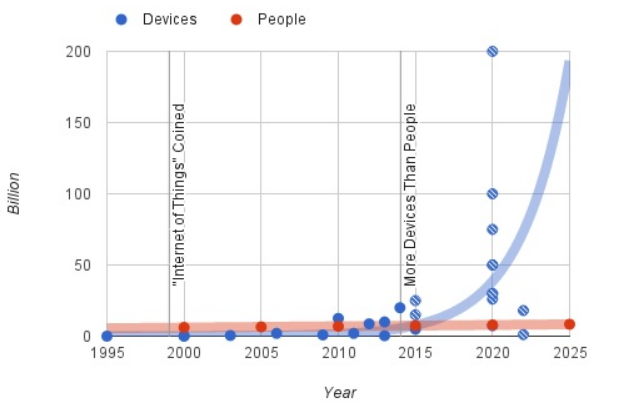
\includegraphics[scale=1]{pic/IoTtrend.png} 
  \caption{Trend of devices vs people \cite{philip2015iottrend}}
\end{figure}

As shown above, recent research from Philip N. Howard \cite{philip2015iottrend} has demonstrated this trend. Between 2011 and 2015 the connected device has experienced exponential growth. 

The concept of IoT is not only a simple extension of Internet. It introduces a way to make physical devices become available in the virtual world. In order to make a real object become a "thing" on the internet, according to Dr. John Barrett \cite{barrett2012IoT}, there are several essential steps to convert an ordinary object in daily life into a smart object in IoT:

\begin{itemize}
  \item First, a unique identifier to tag a thing. Every asset in the IoT has a tag to uniquely identify itself. In this context. IPv6 is the solution for the first step because of its huge volume. Besides IPv6, IPv4 and MAC are also widely being used. However, IPv4 has a fatal limitation of its capacity. With 32-bits space, IPv4 has only 4,294,967,296 addresses which will be used up soon \cite{parkhurst2004routing}. In contrast, the IPv6 has 128-bits space available \cite{parkhurst2004routing}. Similarly, the MAC address is designed to identify a network interface on the physical network level. It has two versions: EUI-48 \cite{guildlinefor48mac2016IEEE} and EUI-64 \cite{guildlinefor64mac2016IEEE}.
  \item Second, the ability to communicate. In order to communicate with the internet, smart objects or called things in IoT must implement a way to communicate. Therefore, different transmission media need different communication mechanisms. Today, we mainly use microwave and twisted-pair as the front end media.
  \item Third, give object senses. In the real world, an object can be identified by smell, feeling, color and so on. It is also true in the digital world. By collecting different data of an object, people can know changes of an object or its surrounding environment. Therefore, people need to implement different kinds of sensors on an object to make it become "smart". By implementing sensors, we acquire desired data of an object to share on the internet.
  \item Fourth, a controller at remote side. Since we can get data from sensors and deliver them to a remote object through the internet, the remote side may have requirements to modify values of a smart object through Internet. Therefore, people need a remote controller to achieve remote control.
\end{itemize}

After above four procedures, objects in real life becomes available as virtual assets in the Internet. As a virtual asset, it can take part in data communication of IoT.

The highlight of IoT is the concept of gathering data from the machine and transmitting data between with pre-programmed procedures, which means less manual operations are required in IoT. In this way, it liberates more productive forces from input data to The Internet to more valuable work. As a basic concept of "smart homes" and "wearable devices", the IoT is a promised coming future. It will make a great influence on our daily life.

In the section, we will discuss the concept of personal cloud which helps us define the edge of proposed architecture.

\section{Personal Cloud} 
The personal cloud is a combination of the private cloud and the public cloud. According to Na, Park and Huh \cite{na2010personal}, "The Personal Cloud describes a user-centric model of Cloud computing where an individual's personal content and services are available anytime and anywhere, from whatever device they choose to access it.". For example, Seagate proposed a personal cloud solution \cite{seagate2016whatispersonalcloud} which aims to provide a centralized media library where a user can access to their data from anywhere. The model consists of software on different platforms and a central server. People can access their digital assets on different platforms through different interfaces but their data are backed up in one physical device. 

In recent years, with the increasing number of personal mobile devices (like smartphones, pads or wearable devices), more and more digital assets are distributed on different devices. For most of the time, those devices are not all in the radiation range of a Wi-Fi network. In this case, those scattered personal devices need to connect to a center node or a bridge device to reach the Internet. Therefore, there are two important facts of a short-range wireless communication technology.

\begin{itemize}
  \item First, the data communication between mobile devices is relatively less intensive than PC to PC communications. It depends on the computing power of mobile devices.
  \item Second, the network state is constantly changing from time to time. It is determined by the nature of short-range wireless communication. 
\end{itemize}

After examining the context of IoT, we found that more and more smart devices are available for a single person. Those smart devices may be placed in a particular place or taken by their owners as portable devices. The personal cloud discovers the requirement of user: Access data at time on any device.

In the next section, we will discuss two popular design styles for the machine to machine communication: SOAP and REST. 
\section{SOAP and REST} 
In general, SOAP is a protocol which was popular in the late 1990s. REST is a design style which has been proposed with HTTP but is not popular until recent years. Technically, SOAP and REST are two different kinds of concept and not directly comparable. Here we put them together just because each of them stands for a style of design.
\subsection{SOAP} 
SOAP is the abbreviation for Simple Object Access Protocol. According to Hadley et al. \cite{hadley2003soap}, it is a "lightweight protocol intended for exchanging structured information in a decentralized, distributed environment". It is a widely adopted protocol for data exchanging among web applications. Both SMTP and HTTP are notable transport protocols which support SOAP well. The format of SOAP message is based on Extensible Markup Language (XML).

\begin{figure}[h]
  \centering 
      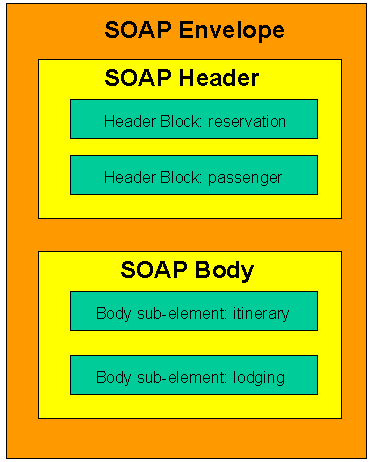
\includegraphics[scale=0.8]{pic/soapformat.png} 
  \caption{SOAP message structure example \cite{mitra2003soap}}
\end{figure}

As shown above, a SOAP envelope consists of two sub-elements: Header and Body. The Header contains metadata which are optional. The Body contains the payload.

The benefit of SOAP is obvious. It allows internet communication between programs with the support of different transport protocols. Meanwhile, because it follows post/response mechanism in HTTP, it can easily pass through firewalls and proxies.

\subsection{REST}
REST stands for representational state transfer. It is proposed by Fielding \cite{fielding2000architectural}. In REST, each available resource at server side can be visited through a consistent path (URI). The client can request different operations (Create, Read, Update, and Delete) through standard HTTP verbs (POST, GET, PUT, and DELETE). Although operations in REST are defined by HTTP verbs, REST is not bound with web service. According to the author, the advantage of REST is obvious because it "emphasizes scalability of component interactions, the generality of interfaces, independent deployment of components, and intermediary components to reduce interaction latency, enforce security, and encapsulate legacy systems". However, those features not just bring benefits but also limitations as well. According to Arcitura \cite{arcitura2016}, there are five constraints for a REST architecture.

\begin{itemize}
  \item Stateless: Stateless is the most important feature of the RESTful design. It indicates that each request from client contains all information a server needs to know, and all session state data should be sent to a client after each request.
  \item Cache: A RESTful design should support cacheable mode by which people can save the latest response for further usage.  
  \item Uniform Interface: It is the fundamental characteristic of a REST service which guarantees each request can independently get an individual resource.
  \item Layered system: An REST-based solution may consist of multiple layers. Communications between service providers and consumers are independent events that can not be affected by changes in other layers.
  \item Code-On-Demand: It is an optional constraint. A client can update its codes independently from a server.  
\end{itemize}
 
The RESTful design makes web application back to the original purpose of HTTP. Since many existing systems adopted SOAP design style, Fowler \cite{fowler2010richardson} proposed three ways towards REST (from a traditional HTTP web service to a RESTful service).

\begin{itemize}
  \item Level 1. Identify every resource: Developers need to design URI to guarantee one to one mapping between resources and URIs.
  \item Level 2. HTTP Verbs: Use appropriate HTTP verbs under different situations instead of using POST only. 
  \item Level 3. Hypermedia Controls: Grant discoverability to response. By adopting hyperlinks in response, users can always get links for next possible operation.
\end{itemize} 

\subsection{REST VS SOAP}
It is common that REST and SOAP are put together to make a comparison.  Theoretically, SOAP is a protocol. It should not be compared with REST. However, those two terms define two popular ways to design services. According to Pautasso et al. \cite{pautasso2008restful}, "REST is well suited for basic, ad hoc integration scenarios,
WS-* is more flexible and addresses advanced quality of service requirements commonly occurring in enterprise computing" (WS-* refers to Web service specifications).
In SOAP, all requests and responses must follow XML standard as well as use the verb: POST. In REST, all four verbs are available and each URLs map to resources. The following section will discuss those two technologies in detail.

\begin{itemize}
  \item Complexity: SOAP adopts XML as transfer format, which means the complexity of serializing and de-serializing is certain. In contrast, REST can adopt different protocols to transfer data. For example, comparing with XML, JSON can store more information with fewer words. On the other hand, in SOAP, operations are all encapsulated in a POST request, which makes it become a black box for users. In contrast, operations in REST are defined by four HTTP verbs. Therefore, the user can easily tell the target resource and action of a request.
  \item Scalability: SOAP was popular when IT services were only available for giant companies. It is designed to fulfill a particular task, which makes codes are hard to scale. On the other hand, REST maps one URL to one resource. It divides complexity of a single page into multiple pages. This characteristic naturally increases the scalability of a system.
  \item Cache: REST is a natural suit for caching. As mentioned above, at the last step towards REST, possible operations of next request are included in the return. In this way, the client-side can easily load and store result before the user makes a request. In SOAP, resources are always wrapped together which makes the next operation of a user is hard to predict. This characteristic makes cache becomes much harder in SOAP.
  \item Security: Because of WS-Security, many people believe SOAP is more secure than REST. However, it is not true. According to Flanders’ research \cite{flanders2009moreonrest}," the WS-* arena certainly has more standards than the RESTful arena (and this will probably always continue to be the case), but there are efforts to support federated security in the world of REST. OpenID is one such effort" (Ws-* refers to Web service specifications). In fact, according to HTTP specification \cite{fielding1999hypertext} only HEAD and GET operations are considered as "safe".
\end{itemize}

In conclusion, we can not simply state SOAP is better than REST or REST is better than SOAP. In order to make a right architectural decision for the proposed architecture, developers need to take more factors into consideration.
\subsection{REST VS SOAP in mobile app}

For a mobile app, where the internet connection is fragile (nature of wireless connection), one single communication between client and server is expected to be short and light.  As mentioned above, compared with SOAP, REST is more lightweight, flexible and controllable. Those characteristics meet the requirement of the wireless connection between mobile devices and the internet. On the other hand, SOAP is not a bad option when mobile apps are used to serve web applications for complex business logic.
\subsection{Summary}

From the analysis above, it is obvious that REST is more simple and clear. In REST, each URI has clear meaning and operations are limited within POST, DELETE, UPDATE and GET. On the other hand, in general, there are more logics in a single page of a SOAP architecture. The XML makes the SOAP can handle complex logics but also increases complexity. In brief, REST prevails over SOAP in lightweight communication. It is especially true at the edge of the network where lightweight payload is required.

After the comparison, I chose REST as the design style of proposed architecture. Since REST is chosen, I turn to explore popular protocols based on REST.
In the next chapter, we will discuss advantages and disadvantages of CoAP by comparing it with MQTT.
\section{MQTT and CoAP}
MQTT and CoAP are two popular protocols in IoT. In this section, we put MQTT and CoAP together to discuss features of CoAP.
\subsection{MQTT}
MQTT stands for MQ Telemetry Transport. It is a lightweight publish-subscribe protocol running on TCP/IP protocol. According to its official website \cite{banks2014mqtt}, "MQTT is a Client Server publish/subscribe messaging transport protocol. It is light weight, open, simple, and designed so as to be easy to implement.".

\subsubsection{Packet Format} 
According to the specification V3.1.1 \cite{banks2014mqtt}, MQTT packet has two bytes fixed header. Therefore, the minimum size of an MQTT packet is two bytes. The following chart shows how an MQTT packet looks like according to the description of the official document.

\begin{figure}[h]
  \centering 
      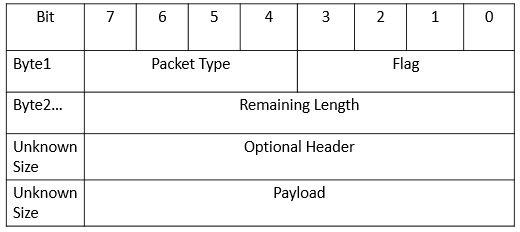
\includegraphics[scale=0.8]{pic/mqttformat.png} 
  \caption{MQTT message format\cite{banks2014mqtt}}
\end{figure}

As shown above, the first byte of MQTT consists of two parts. Bits from 7 to 4 indicate the packet type. Bits from 3 to 0 set flags. Bytes since the second indicate the remaining length of the message. The minimum size of this section is one byte and the maximum is four bytes. After specifying remaining size of a packet, the developer can add optional headers to a packet. After the optional headers, the remaining section of a packet is payload. 

\subsubsection{Feature}
Publisher and subscriber (pub/sub):  In this model, the publisher and the subscriber do not know about the existence of each other. Instead, a broker will gather all published messages from a publisher and accordingly send them to the subscribers after filtering. In other words, there is a central server between publishers and subscribers. In addition, the support of QoS and the Last Will and Testament are two key features of MQTT.
 
\begin{itemize}
  \item QoS: According to Thangavel et al. \cite{thangavel2014performance}, MQTT supports three levels of QoS. At level 0, a message will not be acknowledged or resent by a sender. At level 1, a message will be guaranteed to deliver at least once. At level 2, the receiver will guarantee the message to process. In this case, the sender stores a message and is ready to resend of it. Meanwhile, the receiver stores the reference of a received packet’s id to prevent from processing the same message twice.
  \item Last Will and Testament(LWT): The client can register a LWT when a connection is initialized with a broker. If a client has been disconnected from a broker, the broker will send LWT to all clients subscribed the "lastWillTopic". 
\end{itemize}

In conclusion, the MQTT is a well-designed protocol for lightweight bandwidth. Its logic is simple where all communication between clients is based on message transition of a broker.
\subsection{CoAP}
CoAP is short for Constrained Protocol. It is based on REST model and designed for constrained networks. According to RFC 7252 \cite{shelby2014constrained}, UDP is the default transport protocol for it. Meanwhile, it could also be used over other transports such as TCP. CoAP offers an elegant solution for low bandwidth communication with HTTP-like 

\subsubsection{Packet Format}
CoAP has a four-byte header which includes information of "version", "token", "length of variable-length token field", "message ID" and code of "message type".

\begin{figure}[h]
  \centering 
      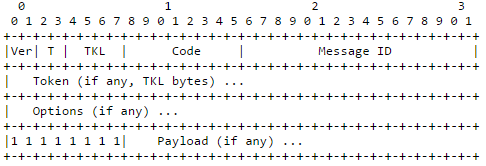
\includegraphics[scale=1]{pic/coapformat.png} 
  \caption{CoAP message format \cite{shelby2014constrained}}
\end{figure}

As shown above, the header of a CoAP message consists of four bytes. 

\begin{itemize}
  \item The first 2 bits of a message shows CoAP version of the message. The following 2 bits indicates message type (4 options available). TKL stands for Token Length (4 bits), which indicates the length of the token field. 
  \item The second byte is "Code" which indicates operation of the message. There are two types of Code. One is called "method code" which consists of 4 verbs in HTTP (GET, POST, PUT and DELETE). The other is called "response code" which returns the result of a request. For example, CREATED, DELETED, VALID and etc. 
  \item The third byte and fourth byte store Message ID.
\end{itemize}

Besides the four-byte header, token and options are additional information which is neither part of header nor payload. The size of token ranges from to 0 to 8 bytes. It is used to match the request and the response. CoAP also supports common used metadata in HTTP. In the Options section, a user can define parameters like in HTTP header, such as Etag, Max-Age, Content-Format, etc. Those options simplify the process of translating COAP messages into HTTP messages.

Unlike MQTT where the remaining length is defined to indicate the length of the optional header and payload size, in CoAP, a 1-byte flag is used before the payload. When a processor first time encounters a 0xFF, it indicates that the payload starts from the next byte.
\subsubsection{Feature}
CoAP has several features. I list the most interesting four as the following:

\begin{itemize}
  \item URI support: CoAP follows a URI scheme which is similar as the one in HTTP.
  \item Similar features to HTTP: Operations in CoAP are based on four HTTP verbs (GET, POST, PUT, and DELETE). Metadata and URI are optional in CoAP. Those two characteristics make it easy to convert messages to HTTP messages 
  \item Resource discovery: "/.well-known/core" is a special URI in CoAP \cite{shelby2012constrained}. By sending request to this URI, a client can get all available resources of a server.
  \item Observation: CoAP supports data observation as an extra option besides traditional "send" and "receive". At server side, a developer can add observable resources to the observer list. Then, a client can register resource observer to get data change notifications.
\end{itemize}
 
From the highlights introduced above, we know that CoAP is a compatible protocol designed for IoT. Although it is efficient, it does not aim to replace HTTP. It is designed to support constrained networks under the consideration of merging them into existing networks. As shown in the following chart, we expect the CoAP to handle medium or small size messages as a bridge between fat web services and low payload networks.

\begin{figure}[h]
  \centering 
      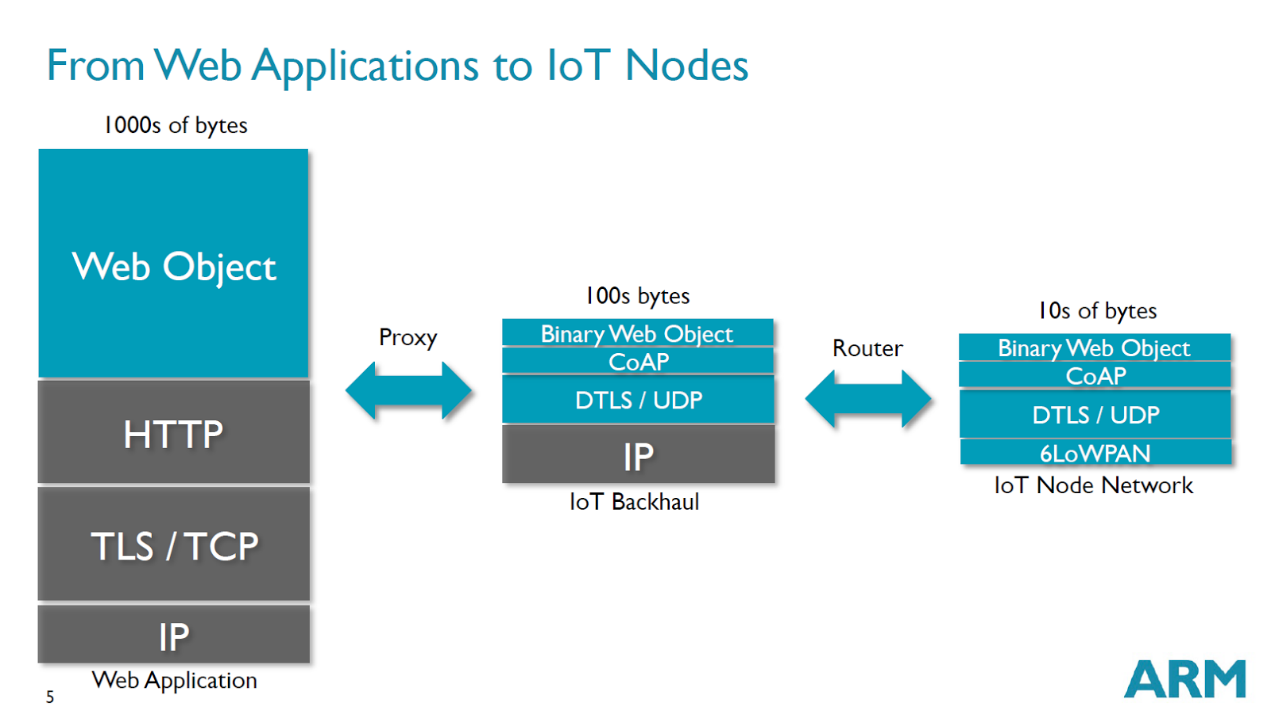
\includegraphics[scale=1]{pic/coapusecase.png} 
  \caption{From Web Applications to IoT Nodes \cite{armcoaptutorial2014}}
\end{figure}

The chart above also shows the current status of IoT network regarding payload size. 
Web applications are the backbone of IoT network. The majority of web applications adopt HTTP. In general, the payload size should beyond 1000 bytes.

Between giant network and IoT nodes, there are routers which act as interpreters between CoAP services and HTTP services. As shown above, attributes in CoAP and HTTP are similar, which minimize works in a proxy. On the other hand, since CoAP is designed for lightweight communication, it can be transferred in channels with lower bandwidth (less than 1000 bytes). Further, at the far end nodes of IoT networks, there are many tiny devices with low bandwidth networks, for example, sensors in a room, iBeacon in a small store, and remote start components in cars.

Besides low-bandwidth, CoAP also consumes less power when compared with HTTP, Colitti et al. pointed out that the power consumption in CoAP is about half of that in HTTP \cite{colitti2011integrating}.

Although UDP is the default underlying protocol to support CoAP, CoAP can be implemented on different protocols. In 2011, Laum et al. \cite{laum2012web} proposed two ways to communicate with WPAN through mobile gateway.

\begin{itemize}
  \item Using 802.1 D standard to connect other 802 projects like Ethernet, Wireless LAN and WiMax.
  \item Using DHCPv6 prefix delegation together with a static routing mechanism to connect other IPv6 based devices. 
\end{itemize} 

Those two methods can support the communication between smartphones and WPAN. Devices in the WPAN need to acquire either 802 structure or IPv6 address.

Similarly, in 2011, Mitsugi et al. \cite{mitsugi2011bridging} proposed a UPnP and ZigBee based solution for CoAP communication between the Internet and constrained networks. In their solution, gateways do not need to translate CoAP messages instead directly deliver them to ZigBee based sensors.  

So far, solutions for implementing CoAP in WPAN assume that sensors have met special hardware requirements. However, in reality, popular technologies like BLE and NFC do not fit the assumption. This fact leads me to explore the possibility of a software layer architecture with better compatibility.

In conclusion, CoAP provides a solution for merging low payload networks into the existing HTTP-based networks. Apparently, it improves the communication between personal networks and the cloud.  
\subsection{COAP VS MQTT} 
Although both CoAP and MQTT can be used as IoT protocols, they focus on different aspect of data transfer.

MQTT, it applies the concept of "client and broker" to replace the concept of "server and client". Since the central hub (broker) is used, it is good for multiple communications between smart machines. Meanwhile, with smaller header, MQTT is more efficient than CoAP in transferring small payload. On the other hand, since it is based on subscription and push model, it expects little data in the payload. In addition, the implementation of "last will statement" makes the protocol with better performance when running in intermittent connectivity. Further, the support of three level QoS makes it a clear solution for reliable communication.

CoAP is designed for HTTP-like communication. A CoAP message can easily be transferred into a HTTP message. One the other hand, the minimum size of a CoAP message is 4-byte which makes it suitable for low bandwidth environment. CoAP does not have a build-in standard to provide quality service, but gives options like "if-match", "if-none-match" and "accept". Those attributes can be used to implement developers’ own strategies for quality service. Similarly, regarding data access mechanism, as mentioned above, the last will statement is implemented in MQTT. However, in CoAP, developers have to take advantages of supported "Etag" and "Max-Age" options to implement their own solutions.

In conclusion, the MQTT aims to support multiple clients’ communication within a small network. The CoAP focuses on REST communications and the communications between small networks and the Internet. The CoAP is more flexible and closer to HTTP protocol. In addition, it is more friendly to developers. At last, it requires less effort to transfer a HTTP service into a low bandwidth network. 
\subsection{Summary}
In the above section, I compared two most popular technologies in IoT. According to the analysis, I draw the conclusion that CoAP is closer to the Internet than MQTT. If I plan to design an architecture where messages can easily be transferred into HTTP messages, I should adopt COAP.  As mentioned in the problem definition, our goal is to accelerate the process of merging NonIP based devices into IoT. So, I decide to choose CoAP.  

Since I decided to use BLE as an example to test the proposed architecture, I need to review associate works of BLE. In the next chapter, the paper will discuss strength and weakness of Bluetooth and Bluetooth Low Energy.

\section{Bluetooth}
Bluetooth is a standard for low bandwidth wireless communication. It is maintained by the Bluetooth Special Interest Group (SIG). The latest version of Bluetooth is 4.2. The BLE has widely been implemented in smart devices like tablet, smartphone, and wearable devices. It is designed for networks with low data payload but needs frequent small data transfer. It is invented in 1994. Originally, "Bluetooth was designed was conceived as a wireless alternative to data cables by exchanging data using radio transmissions" \cite{Bluetooth2016SIG}.

So far, Bluetooth consists of four technologies: Bluetooth, Bluetooth EDR, Bluetooth HS and Bluetooth low energy. Since Wi-Fi takes great advantages in the field of high-speed data transfer, SIG focuses more on lightweight and low energy communications. In version 4.0, the SIG proposed "Bluetooth Low Energy" to take up the market of low energy wireless communication.

In the remaining section of the chapter, I will discuss the differences between class Bluetooth and Bluetooth low energy. Further, I will explore relevant works of BLE.

\subsection{Classic Bluetooth}
As mentioned above, Classic Bluetooth is a reference of Bluetooth 2.1 or below. It is designed for streaming data transfer. It adopts Standard Bluetooth Profiles (SPP, DUN and PAN) where one master device can have up to seven slaves. Communication through Classic Bluetooth is based on data streaming. In this way, the Classic Bluetooth has better data rate but less energy efficiency. 

As shown in the following figure \cite{bluetooth2010bluetooth}, in a BR/EDR piconet, two or more devices occupy the same physical channel. Messages in a physical channel are synchronized by a common clock and hopping sequence. A Bluetooth can not be a master of more than one piconet, but it may belong to two or more piconets. In the following figure, the device A is a master of a piconet with device B, C, D and E as slaves. Meanwhile, the device D is a master of another piconet with J as the slave. The device E plays a role of slave in both the piconet of A and F. The K is an isolated advertising node.

\begin{figure}[h]
  \centering 
      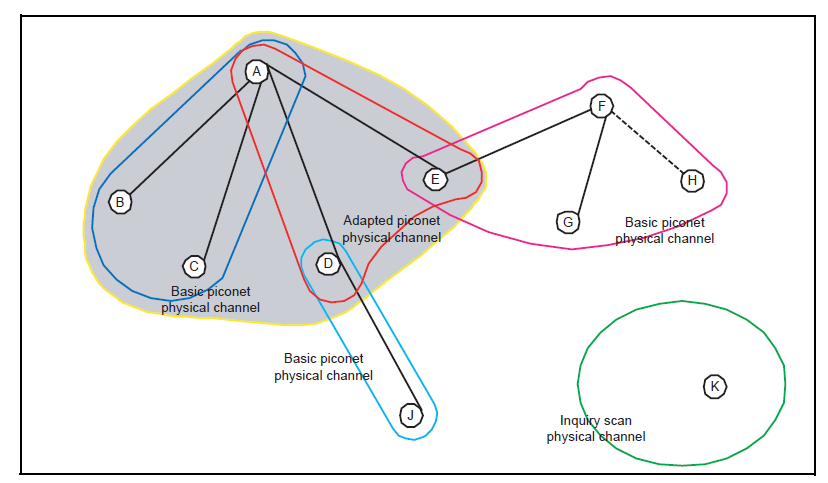
\includegraphics[scale=0.6]{pic/classicbluetoothtopology.png} 
  \caption{Topology of Classic Bluetooth \cite{bluetooth2010bluetooth}}
\end{figure} 

As mentioned above, the classic Bluetooth has widely been adopted in wireless communications. However, it has a natural disadvantage. Since wireless communications are built-in fragile, the streaming data can be interrupted at any time. Moreover, in a single piconet network, one master device can only be connected to up to seven slave devices. Those limitations have impeded the development of it. On the other hand, in 1997, Wi-Fi is introduced. And, the data rate of Wi-Fi reached 11Mbit/s \cite{lan2003part}. With the development of Wi-Fi, it gradually overlaps the use cases of Bluetooth with better data rate. For example, a research from Friedman et al. \cite{friedman2013power} shows the advantage of Wi-Fi in smartphones’ file transfer. After the attempt of increasing data rate in version 3.0, the SIG turns to develop low-energy version of Bluetooth. 

In conclusion, the class Bluetooth is a success product. However, it can not make a breakthrough when facing the challenges of Wi-Fi. The future of Bluetooth has turned out to focus on support smart devices by adopting BLE. In the following section, we will discuss BLE.
\subsection{Bluetooth Low Energy}
The concept of Bluetooth Low Energy is introduced since Bluetooth 4.0. It is designed for low-cost data communication. According to Litepoint \cite{BLE2014litepoint}, the new low energy technology of Bluetooth supports short data packages with the speed of 1Mbps. In addition, it supports fast transactions as short as 3ms. 


\begin{figure}[h]
  \centering 
      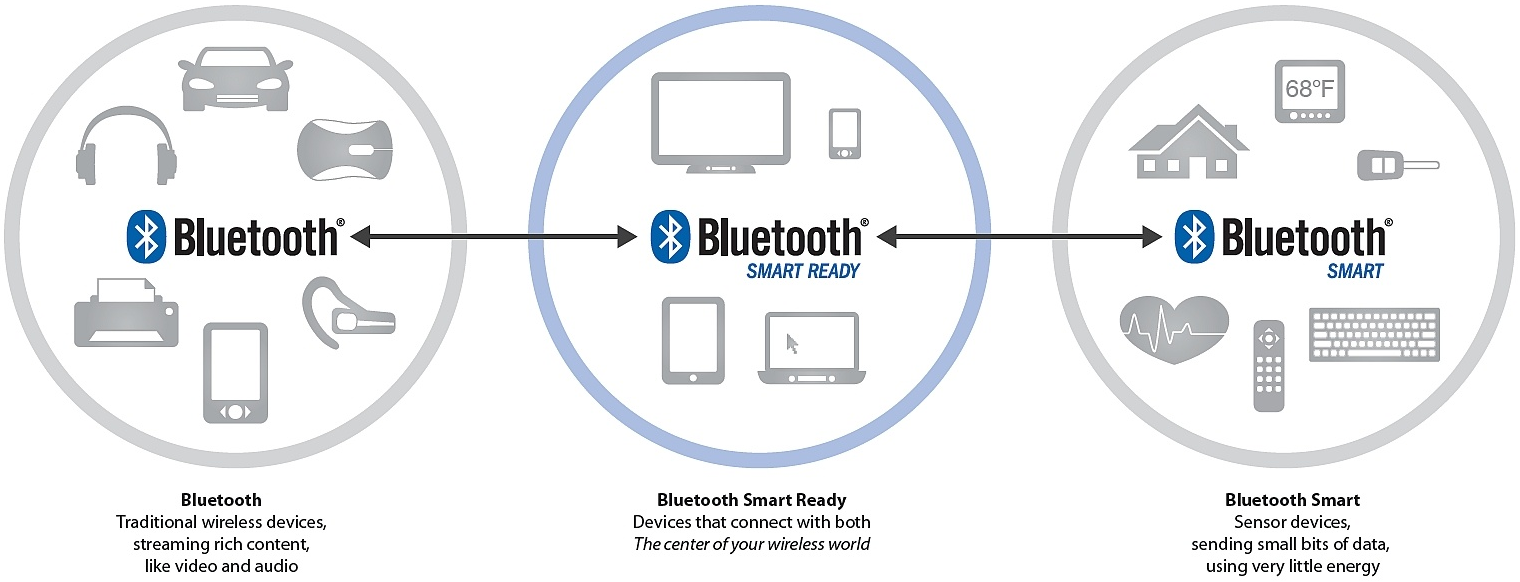
\includegraphics[scale=0.4]{pic/bluetoothproductsrelationship.png} 
  \caption{The relationship between Bluetooth Smart and Bluetooth Smart Ready devices \cite{torvmark2013threeflavourofbluetooth}}
\end{figure} 

As shown above, so far, there are three kinds of Bluetooth devices ("Bluetooth", "Bluetooth Smart Ready" and "Bluetooth Smart"). Devices with "Bluetooth" logo only supports Classic Bluetooth connection. If a Bluetooth device can communicate with both Classic Bluetooth devices and BLE device, it is named as " Bluetooth Smart Ready ". At last, those devices that only support BLE are called "Bluetooth Smart". 

As shown below, unlike classic Bluetooth communication between BLE devices is based on GATT (Generic Attribute Profile) and ATT (Attribute Protocol). According to Bluetooth4.0 specification \cite{bluetooth2010bluetooth}, "The GATT server sends responses to requests and when configured, sends indication and notifications asynchronously to the GATT client when specified events occur on the GATT server.". As shown in the following figure, a GATT profile may contain one or more services. Each service acts as a folder to contain a set of characteristics to store data. For a characteristic, there are three types of attributes: "Properties", "Value" and "Descriptor". The BLE client can read, write or monitor the "Value". 

\begin{figure}[h]
  \centering 
      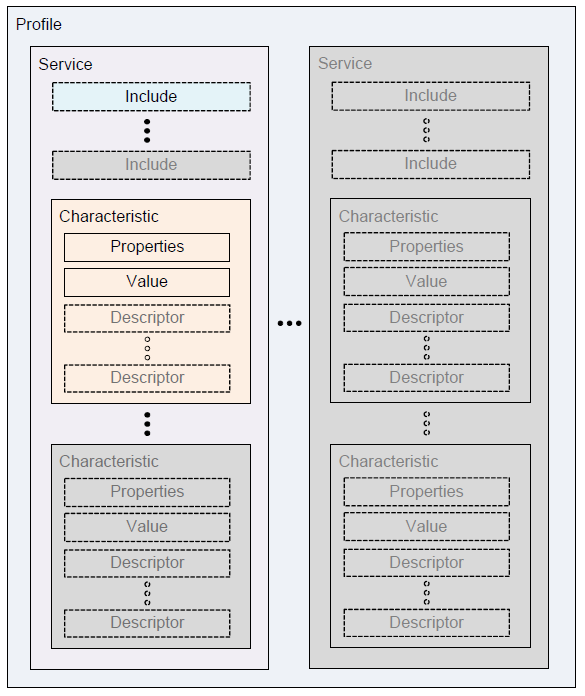
\includegraphics[scale=0.6]{pic/gattformat.png} 
  \caption{GATT format \cite{bluetooth2010bluetooth}}
\end{figure} 

As shown below, there is a great difference between Classic Bluetooth and Bluetooth Low Energy in terms of topology. In BLE, one physical channel consists of two devices, which means each slave communicates with a master in a separate physical channel. 

\begin{figure}[h]
  \centering 
      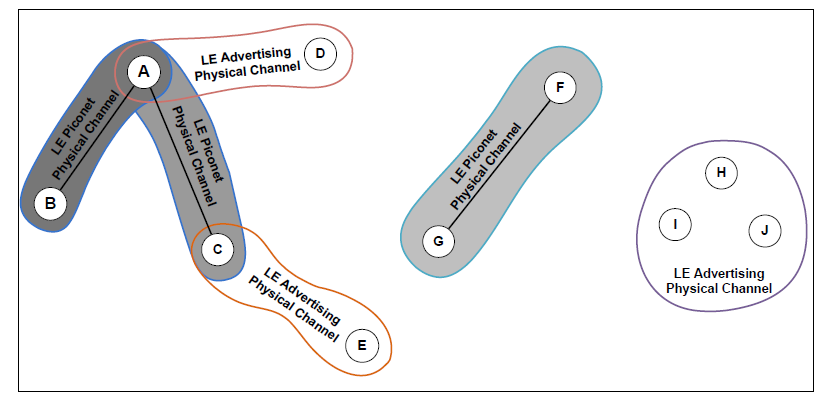
\includegraphics[scale=0.6]{pic/bletopopogy.png} 
  \caption{Topology of BLE \cite{bluetooth2010bluetooth}}
\end{figure} 

So far, there are two more versions available for BLE. The first update is available since 2013 (called Bluetooth 4.1). The second update is available since 2014 (called Bluetooth 4.2).
\subsubsection{Bluetooth 4.1} 
There are four main changes in version 4.1 \cite{SIG2013updaebluetooth4.1}.

\begin{itemize}
  \item Solve interference: Bluetooth and LTE interfered with each other. In this version, it tries to prevent the interference between them.
  \item Flexible Connections: Bluetooth 4.1 allows manufacturers to customize reconnection timeout intervals, which helps to reduce power consumption.
  \item Multiple roles: Devices can act as hubs and end points at the same time.
\end{itemize}

Jawanda \cite{SIG2013updaebluetooth4.1} pointed out that "We updated the Bluetooth specification to address this projected growth, making changes to give developers more control in assigning a role to their product, limiting interference with other wireless technologies, and allowing Bluetooth Smart products to exchange data faster and maintain connections with less manual intervention.".
\subsubsection{Bluetooth 4.2} 
The latest version of Bluetooth is 4.2. According to FAQ document of Bluetooth \cite{SIG2014bluetooth4.2faq}, the latest version has improved BLE in three aspects: IoT capability, security, and speed. 

\begin{itemize}
  \item Regarding IoT capability, a BLE device can directly participate in IoT network by adopting 6LowPAN and connect with routers supporting Bluetooth Smart Internet Gateway. 
  \item Regarding security, LE Privacy 1.2 was introduced to prevent Bluetooth smart devices being tracked by untrusted devices. Moreover, it uses FIPS-compliant encryption to secure data transfer.
  \item Regarding speed, the SIG claims the new patch will make BLE 2.5 times faster and capacity of packet will be 10 times larger than previous versions. 
\end{itemize}

\subsubsection{iBeacon} 
iBeacon is a protocol proposed by Apple. It defines the usage of BLE in goods’ information transfer. According to BLE’s advertising standard, users can set up to 20-byte payload. Apple proposed the protocol to format advertising data \cite{iOS2014ibeacon}. The 20-byte are divided into three parts: 16-byte UUID, 2-byte major value, and 2-byte minor value. The protocol is designed for business owners who want to push ids of their products to people who are nearby around the store. The technology takes the advantages of BLE’s advertising mechanism which can guarantee that those 20 bytes can always be pushed to BLE smart ready devices. 
\subsubsection{6LowPAN}
6LowPAN is short for IPv6 over Low-Power Wireless Personal Area Networks. So far, the latest version of BLE \cite{SIG2014bluetooth4.2faq} has proposed 6LoWPAN implementation and Bluetooth Smart Internet Gateways to support IPv6 based communication. This means that a remote device can directly control a BLE sensor through IPv6. The 6LowPAN is designed for low cost implementation of IPv6. A research from Chawathaworncharoen et al. \cite{chawathaworncharoen2015feasibility} shows that "the power consumption of 6LoWPAN over BLE is one-tenth lower than that of IP over WiFi". In addition, Kovatsch \cite{kovatsch2010embedding} pointed out that "The low-cost, low-power 6LoWPAN modules can easily be embedded into inexpensive small appliances as well as battery-powered controllers like sensor nodes or mobile light switches". According to the analysis from Ma et al. \cite{ma2008analysis}, "Because of its cheapness and practicality, 6LowPAN displays the great market foreground.".

\begin{figure}[h]
  \centering 
      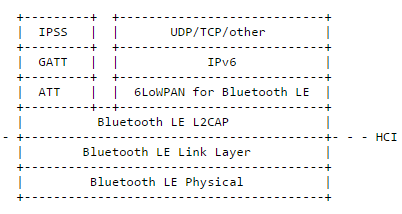
\includegraphics[scale=1]{pic/ble6lowpansolution.png} 
  \caption{IPv6 and IPSS on the Bluetooth LE Stack \cite{nieminen2015ipv6}}
\end{figure} 

As shown above, the 6LowPAN works in parallel with the original GATT protocol stack. At application layer, it can support different languages which are not limited in UDP and TCP. The adoption of 6LowPAN will accelerate the integration between BLE and the IoT.
\subsection{Classic Bluetooth vs Bluetooth Low Energy}
Based on above introduction, we can draw a conclusion that Classic Bluetooth and Bluetooth Low Energy target different markets. For Classic Bluetooth, it is a desirable solution where higher data rate is required and more power is available. For Bluetooth Low Energy, it is designed for devices with less power than Classic Bluetooth devices. BLE is a better option where small amount of data need to be transferred frequently. Also, the BLE it different from Classic Bluetooth. This conclusion can be supported by the research from Rolf Nilsson and Bill Saltzstein \cite{nilsson2012bluetooth}. They pointed out that "Bluetooth low energy technology does not replace Classic Bluetooth technology—it is a whole new game"
\subsection{Summary}  
So far, the BLE is widely adopted in smart devices, which has strengthened its position in the market. With the adoption of IPv6, it can join the IoT with little effort. Meanwhile, with more and more extra protocols are developed (e.g. iBeacon), the ecosystem of BLE will become more and more robust. The latest changes for BLE are IPv6's capability, packet size and security level. Those improvements meet the evolution of IoT. Bluetooth needs to become more compatible with existing networks and transfer more data in a more secure way.  With the development of IoT, it is expected that both the density of sensors and the computing power will increase. In recent BLE have two innovative directions:

\begin{itemize}
  \item The first direction goes toward: BLE devices become cheaper and simpler. This kind of sensors aim to collect limited amount of data. For example, in a large farm land, the farmer needs to manage temperature and humidity in different spots. In this scenario, many sensors will be involved in the network. They will constantly report two types of data to the local hub. In this case, each sensor needs to be as cheap as possible.  
  \item The other direction is: integrating sensors in smart devices, where different kinds of data are processed at the same time. Therefore, this type of devices is constrained by both battery and bandwidth. The recent updates improved BLE’s performance. Now, developers are more comfortable to develop medium size apps based on integrated sensors.
\end{itemize} 

In the next section, I will discuss the CAP theorem which becomes a principle guiding the design and implementation of the proposed architecture.
\section{CAP Theorem}
The CAP stands for Consistency, Availability, and Partition-tolerance. It is an important concept in any design of a distributed architecture. It was first proposed by Brewer in 2000. In 2002, Seth Gilbert and Nancy Lynch proved \cite{gilbert2002brewer} the theorem and pointed out that "It is impossible to achieve all three.". The following are details of those three concepts:

\begin{itemize}
  \item Consistency: Consistency means operations can only be fully executed or dropped.
  \item Availability: Availability means a user can be served at any time. For example, a high availability system can be accessed by users at any time even when it is updating or maintaining.
  \item Partition Tolerance: A system with high partition tolerance can still serve users even if connections between two nodes are lost.
\end{itemize}  

Since the intermittent connectivity is a given condition, mobile applications must achieve high partition tolerance. Therefore, the options for a mobile application are limited between PC (Partition Tolerance and Consistency) and PA (Partition Tolerance and Availability).

In the context of PA (Partition Tolerance and availability), the system and database are separated into different nodes to guarantee both Partition Tolerance and availability. Since the whole data assets are available for each node, a user can access any data when one or more nodes are not available. However, in this scenario, consistency cannot be guaranteed since changes made by the user need to synchronize with the lost node only when the network is available.

In the context of PC (Partition Tolerance and Consistency), if a system’s Consistency is required while the system needs partition tolerance, the system can not have high availability. When a node lost connection, other nodes can change data without worrying about the issue of inconsistency. However, in this scenario, users can not access data in the lost node. 

The proposed architecture aims to guarantee high availability.  Even if a connection between devices are not available, a request should get a response. Therefore, the system must choose PA as its design principle.

\chapter{Architecture}
With the development of smart devices, the fragile network of sensors becomes more and more reliable. Under this context, we expect the CoAP should be supported in those networks. In this research, our main goal is to propose a suitable solution to support CoAP in Non-IP based WPAN.  

Currently, implementations of CoAP only support IP based communication. Technologies like BLE (below v4.2) and NFC do not support IP and have their own standards to transfer data. However, with the development of WPAN and CoAP, it is time to think about the possibility to grant CoAP in WPAN. In addition, if CoAP is adopted as a general protocol in WPAN, it can simply the data communication between WPAN and existing networks.

In the remaining section of this chapter, we will introduce our solution: CoAPNonIP architecture.  

As shown below, the proposed CoAPNonIP architecture consists of an application layer and a network layer. The application layer focuses on message management and message delivery.  

\begin{figure}[h]
  \centering 
      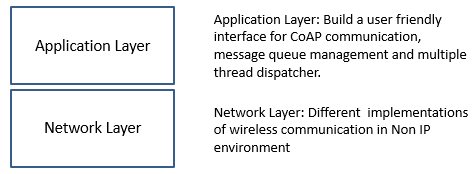
\includegraphics[scale=1]{pic/designlayers.png} 
  \caption{Layers of proposed architecture}
\end{figure} 

\section{Application Layer}
I would like to thank my colleague XiaoDan.Li who has involved in the implement and design of application layer.
In order to provide an easy-to-use tool for developers, we adopt an application layer to manage data and provide a user-friendly interface. 

\begin{figure}[h]
  \centering 
      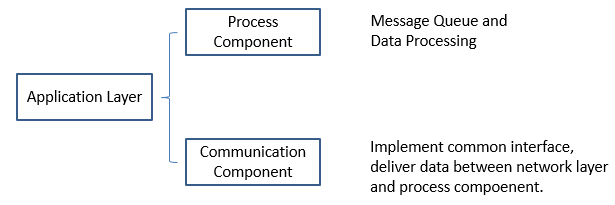
\includegraphics[scale=1]{pic/designapplicationlayer.png} 
  \caption{Application layer structure}
\end{figure} 

As shown above, in order to make sure the proposed architecture have the capability of supporting different protocols of WPAN and providing a robust management mechanism, we have implemented two components in the application layer.  The process component aims to provide queue management for sending and receiving messages. The communication component aims to provide a common interface for message delivery between current layer and network layer. 
\subsection{Process component}
The process component aims to provide a message management hub where message queue and cache are implemented. In the process component, important concepts are listed below: 

\begin{itemize}
  \item Receiver: Receiver is the access point of received data.
  \item Sender: Sender is a thread to convert objects to a byte array and send it to the network layer.
  \item Processor: The processors consist of multiple processor threads where specific CoAP request can be processed in a predefined way.
  \item Resource: Resource keeps the original concept in CoAP. It represents an available data value at server side. A resource management tool is provided in the application layer.
  \item Callback Map: When a user tries to send a request, he or she can specify a customized callback function to handle responses, which will be registered in a callback map for management.
  \item Default Receive Handler: If users do not specify a callback function for a request message, a default response handler will be triggered when a response comes.
\end{itemize}

The main task of process component is to manage resources and handle messages. To increase the efficiency of the system, we grant the architecture the ability to define multiple threads to process data. In detail, users can define one or more processors to process received data and one or more senders to send data. 

\begin{figure}[h]
  \centering 
      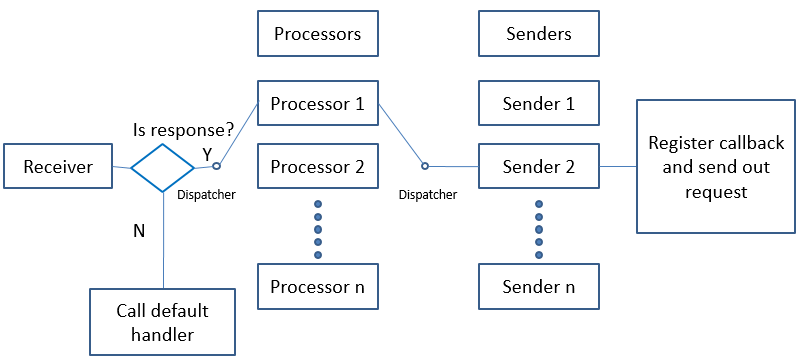
\includegraphics[scale=0.8]{pic/processcomponentflowchart.png} 
  \caption{Process component flowchart}
\end{figure}

As shown above, there are three important roles in application layer: Receiver, Processor, and Sender. When a receiver gets messages from the network layer, it will trigger a callback function which is defined by the developer. If the call back function needs to process the received message, it will run a dispatcher to decide which processor to process the data. After processing the data, a response may need to be sent.

\subsection{Communication component}
Messages received and sent in process component are based on function calls at communication component. The communication component implements a general interface where following actions are defined:

\begin{itemize}
  \item Broadcast: if a device wants to become a server in WPAN, it needs to broadcast itself to make sure other devices can find it. When a device is broadcasting itself, it is in discoverable state. Regarding BLE’s implementation, this broadcast method will try to claim the device as a BLE advertiser.
  \item Search Peers: If a device plays the role of a client, it needs to search nearby broadcast signals to find other nodes. Regarding BLE’s implementation, this method triggers a search operation. If a searcher finds a broadcaster and creates a connection with it, the searcher becomes a central device.  
  \item Get Nodes: A node needs to know available devices in its network to decide destinations of a message. Regarding BLE’s implementation, this method returns all connected devices.
  \item Send Data: Nodes may send data to one or multiple target devices. Regarding BLE’s implementation, this method sends CoAP message and its destinations to network layer.
  \item Receive Data: Nodes need to receive data from remote devices. Regarding BLE’s implementation, this method receives data through call back function.
\end{itemize}

The communication component is implemented based on the technology used at the network layer, which grants the architecture’s reusability. Meanwhile, since the interface only consists of five functions, it guarantees low coupling.

From descriptions above we know that the application layer consists of two layers. The process component proposes a multiple thread mechanism to manage messages.  It grants more efficiency to the whole solution. Meanwhile, by supporting default handler and customized handler, it defines a standard procedure to handle CoAP messages. 

The communication component defines an interface for five common functions. For different technologies, there are different ways to implement those functions. However, the definitions of those functions set standard actions for communication. In practice, based on those five basic functions, developers can customize more actions to meet a specific requirement. In this way, this component provides great flexibilities as well as basic principles.

To sum up, the application layer introduces two components to handle messages, support multiple communication technologies and provide the capability of processing and sending data.

In the next section, I will explain the detail design of network layer for BLE.
\section{Network Layer} 
In the proposed architecture, the network layer is the underlying layer for communication. 
The main task of network layer is to transfer data between application layer and connected devices. The network layer has different implementations for different protocols. 

Under the context of BLE, I create a background service as network layer to serve the application layer. The service receives messages from the application layer and chops messages into multiple 20-byte packets before sending them out. Meanwhile, it retrieves data from remote devices, assembles them into CoAP messages and delivers those messages to the application layer.

At network layer, a device can act either as a server service or a client service. If a device decides to search other devices’ signals, it will act as a client service. Otherwise, it will broadcast itself as a server service. Since the communication between network layer and application layer is based on broadcast, network layer can easily send messages to multiple applications.

If the device acts as a server, it will create a thread to loop message queue for sending out messages and an instance to register callback functions. Meanwhile, the server defines two characteristics for receiving and sending data respectively. On the other hand, if a device acts as a client, it will try to connect with the nearby server. A client maintains a send thread for each connection. 

In the following section, I will discuss the communication mechanism of client and server in details.
\section{Detail Design} 
In this section, I will explain details of proposed two-layer structure.
\subsection{Application layer}
As mentioned in the previous chapter, the application layer consists of process component and network component. In the following section, more details are discussed below.  
\subsubsection{Process Component}
The process component defines how users communicate with underlying architecture. Instead of dealing with message delivery or pruning messages into appropriate format, it focuses on loading balance as well as role determination. There are five basic functions in the component:

\begin{itemize}
  \item "InitReceiver": In this function, developers define actions when CoAP messages are received by application layer. If developers do not want to customize the handler for receiving data, the architecture will send received messages to a default handler.
  \item "InitProcessor": By calling this function, a developer can create numbers of threads to handle received CoAP requests. Those threads will execute predefined actions for each resource. 
  \item "InitSender": By calling this function, a developer can create one or more threads to send out messages.
  \item "SetDefaultResponseHandler": The user needs to provide a default handler for coming request which does not have predefined process.
  \item "Run": After complete all necessary initial settings, the developer can start the CoAP service with different parameters. I defined four different roles to start-up a service.
\begin{itemize}
\item Broadcaster: The device will advertise itself and wait for connection requests from remote devices. 
\item Seeker: The device will search nearby broadcasters to create a connection with it. 
\item Auto: The device will try to find an available broadcaster in limited time. If no broadcaster is found in time, it will turn to broadcast mode to broadcast itself.  
\end{itemize}
\end{itemize}

\subsubsection{Communication Component}
As mentioned above, I define three events and six abstract functions in the network components. The architecture defines three kinds of events: peer found, peer lost, and data receive. Developers can either handle those events at communication level or expose them to process component. Regarding functions, the architecture defines actions for broadcasting, searching peers, sniffing peers, getting nodes, sending data and receiving data.
\subsection{Network layer}
As mentioned above, in the proposed architecture, a device can either acts as a client or a server. A client or a server encapsulates its communication mechanism in a service which runs at background to serve multiple apps. 

In the following section, I will discuss the detail design of client side and server side separately. 
\subsubsection{Client Side}
As mentioned above, the client side runs independently as a background service. It serves one or more apps through message broadcasting. The service can automatically search nearby available servers and connect with them. Whenever a client service gets an available server, it will create a new thread to communicate with the server. The client service will maintain each communication thread in a list. A communication thread will not only listen to events from the remote side but also maintain a message queue to send data. 

A client service will listen to two kinds of messages from the upper layer: announcement and data. (announcement is a special type of message, which is designed for information exchange when a connection is initialized) The communication mechanism will be introduced in a separated chapter. Since the size of a CoAP message can easily over 20 bytes, the service may need to split one CoAP message into multiple packets before sending to BLE channel. 

On the other hand, the client service will handle events of a communication channel by creating three handlers: "OnMessageReady", "OnReceiveAnnouncement" and "OnLostConnection". 

\begin{itemize}
  \item The "OnMessageReady" will be triggered when a complete CoAP message is received. 
  \item The "OnReceiveAnncouncement" will be triggered when an announcement is received. Since the architecture forces client and server to exchange announcement whenever they establish a connection, the architecture also regards it as a signal of connection created. 
  \item The "OnLostConnection" will be triggered when a connection is lost.   
\end{itemize}

Regarding sending and receiving messages, when messages need to be sent, the client side will write data to the "InCharacteristic". Meanwhile, the client listens to the "OutCharacteristic" to get data from server side.

The service also maintains a receiver. As soon as get a message from the remote side, the receiver will retrieve its type. If the message type is 0 (an announcement), the receiver will construct an object with information of remote UserID, remote AppID, and remote mac address. In addition, the receiver will trigger an announcement-received event where constructed object is the parameter. If a message type is 1 (a subsequent packet), the receiver will add the received message to a hashmap where the combined string of UserID and AppID is the key. The hashmap maintains messages received from the connected device. If the message type is 2 (the end packet of a CoAP message), the receiver will add the message to the hashmap, combine existing message pieces into an object and trigger a message-received event.  
\subsubsection{Server Side}
As mentioned above, the server side runs independently as a background service. It serves one or more apps through message broadcasting. A server broadcasts itself and remote clients can connect with it. Once a connection is created, connected devices can read and write values to the server. 

Similarly, the server-side listens to the request of sending announcements or messages from upper layer. When new request is received by the service, it will process the data and push data packets to a queue. A sending thread manages the queue and constantly sends data. 

Regarding sending and receiving messages, the server service listens to the value of "InCharacteristic" to get data changes. Meanwhile, when data need to be sent, it will change the value of "OutCharacteristic" and send a notification to the client side. 

The server side also supports three types of messages which have been described earlier. Once the message is received, the server-side needs to parse it into an object and trigger a message received event.

In the flowing section, I will use two flowcharts to explain how service works and how messages are processed. 
\subsubsection{Flowchart}
The flowchart below shows the lifecycle of a service. As shown above, whenever the user creates a CoAPNonIP service, he or she needs to create an instance of an object called App. At the time of initializing the App, logics at application layer need to be specified. After calling several functions to initialize the application layer, users need to call "Run" function to start the service. If no service is running at background, a new service will be created. The service keeps running until the user forces to stop it.

\begin{figure}[H] 
  \centering 
      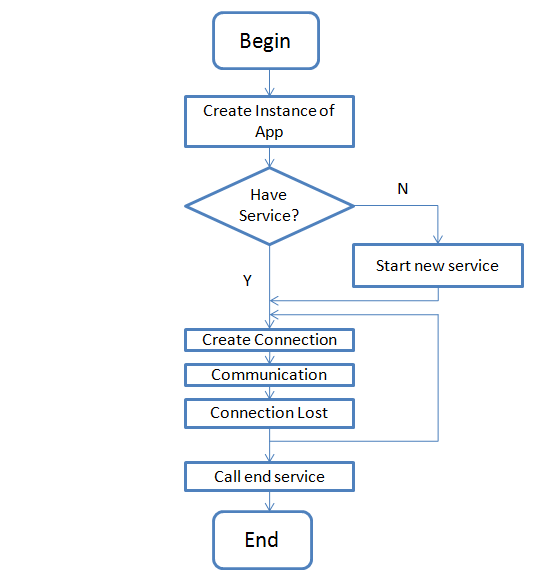
\includegraphics[scale=1]{pic/networklifecycle.png} 
  \caption{Life cycle of network service}
\end{figure} 

The flowchart below shows the life cycle of communication. Since the architecture is resource driven, a request needs to specify the resource URL and targets. After creating a request, the system will send the message to the sender queue and register a handler for handling response. Sender thread sends messages to network layer service. In the service, the program decides whether the communication channel is available before sending data.  When a request is received, the network layer of remote device will throw it to the application layer. In the application layer, messages will be pushed into processor queue. When a processor thread retrieves messages from the queue, it will judge whether target resource is available. If the resource is available, the system will execute operations, generate a CoAP response and send the response back. Finally, in the application layer of request sponsor, the program will try to find a handler in the hashmap (key value pair of message id and handler) to handle the response.

\begin{figure}[H]
  \centering 
      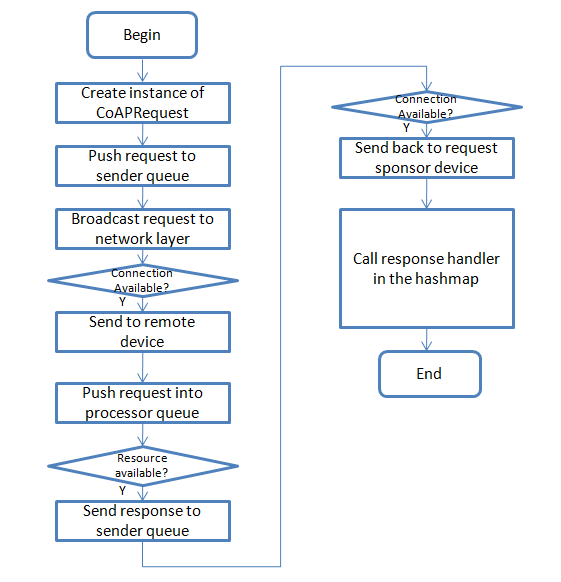
\includegraphics[scale=1]{pic/communicationlifecycle.png} 
  \caption{Life cycle of network service}
\end{figure}

\subsubsection{Packet Format}
As shown below, in the proposed architecture, a protocol is designed based on 20-byte BLE packet.  The protocol consists of two parts: 4-byte header and 16-byte payload. 

In the header, the first 2 bits indicate the type of the packet. Currently, there are three types available. 

\begin{itemize}
  \item "00" stands for announcement: Announcement message is a special type of message which only has 4-byte header. It is used to exchange AppID and UserID.
  \item "01" indicates that the packet is a continued packet, and the service should expect more packets and assemble them into a CoAP message.
  \item "10" means that the last peace of a CoAP message is received.     
\end{itemize}

The following 14 bits are used by AppID. It defines which apps are sending the request. The range of the number is from 1 to 16383. 

The remaining 16 bits are used by UserID is used to indicate which user is sending data.  The range of it is from 1 to 65535. 

Since header has 4 bytes, the remaining 16 bytes are used as payload to carry the CoAP messages.

\begin{figure}[H]
  \centering 
      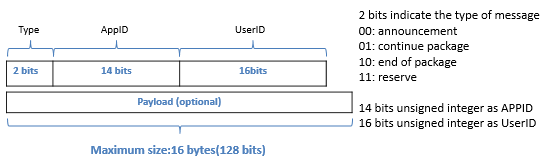
\includegraphics[scale=1]{pic/packetstructure.png} 
  \caption{Packet structure}
\end{figure}

\subsubsection{Communication Mechanism}
As introduced in the literature review, BLE’s communication mechanism is not stream based. Instead, a BLE connection is open and close periodically. Messages are only sent out in short time frames when the connection is open. There are two ways to send a message in BLE: One is to send a message sequentially, which will wait for a signal from a remote device before sending the next message. The other is to send messages without waiting responses from the remote device. The proposed architecture sends and receives messages sequentially. The following chart shows how BLE client and server communicate with each other.

\begin{figure}[H]
  \centering 
      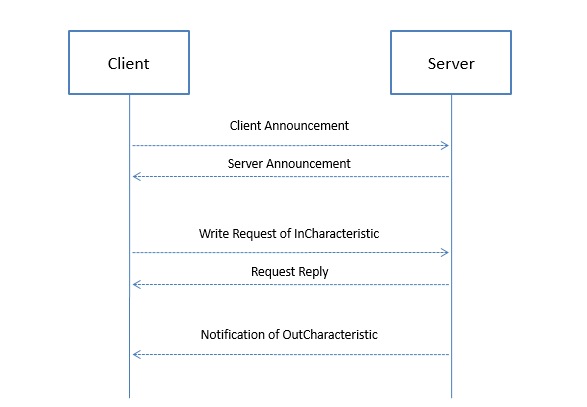
\includegraphics[scale=1]{pic/communicationmechanism.png} 
  \caption{Communication mechanism}
\end{figure}

As shown above, once a connection between devices is created, the client side will send one or more announcements to the server side. Meanwhile, the server side will send an announcement to the client. Once the announcement information is exchanged, client side can write characteristics at server side to send a message. Meanwhile, server side can send a message to the client through notification.

The announcement is introduced as a "shake hands" mechanism before communication. Unlike AppID and UserID in other messages, AppID and UserID in an announcement are values of the source device. In this way, before sending any information, each side can know the role of the device. Since the architecture uses AppID and UserID fields in two different ways, it can overcome the chaos of message received at the server side as well as act like utilize them as unique IDs to filter messages for different applications. After "shake hands", messages between two devices must be sequential, which means both sides need to wait the received signal of previous BLE packet before sending a one.
\subsubsection{Virtual Resource}
In standard CoAP protocol, all requests and responses are RESTful. In this context, resources are bound on one device. However, one device may need to gather the same type of same data from different devices. Since more and more cheap sensors are available in the market, this kind of requirement will increase. 
Therefore, in the proposed architecture, a virtual resource mechanism is proposed to meet the need of multi-sampling. The virtual resource is achieved by introducing a timer to wait for return values from connected devices.

\begin{figure}[H]
  \centering 
      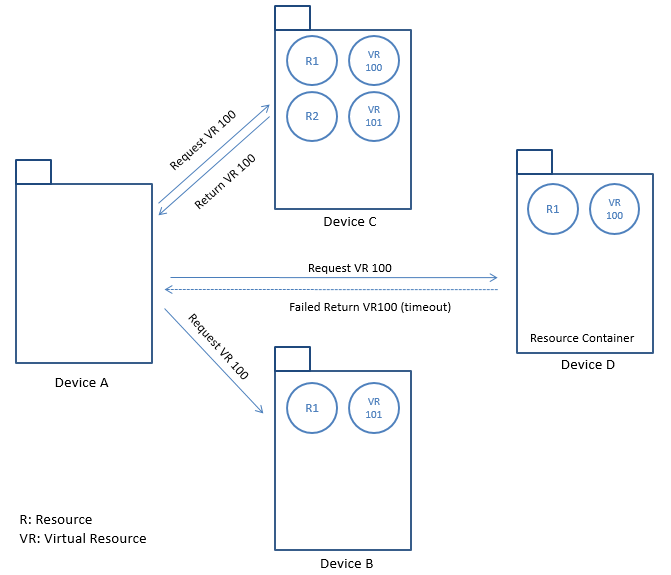
\includegraphics[scale=0.8]{pic/virtualresourcemechanism.png} 
  \caption{Virtual resource mechanism}
\end{figure} 

As shown in the above chart, in the view of resources, all involved devices are resource containers. The device A broadcasts a request (requiring the value of virtual resource 100) to all connected devices. The device B does not respond the request because resource 100 is not available. The device C successfully returns the value of resource 100. The device D has resource 100 but it did not respond in time. Therefore, the device A will receive one return.

\section{Proposed Solutions for Problems}
In the following sections, I will discuss solutions for problems mentioned in problem definition section.
\subsubsection{Identify Non-IP based devices}
The proposed architecture adopts the concept of AppID and UserID. As mentioned above, an application can get a unique identifier by combining those two numbers together. In this way, the architecture has a software layer ID to identify services. In the physical layer, devices may have MAC address, IP address or another way to identify itself. However, all devices in the proposed architecture need to use AppID and UserID to identify themselves. One advantage of this design is that the system can easily change devices with less effects on. Moreover, the adoption of AppID and UserID grants flexibility to the architecture if multiple communication technologies need to be supported at the same time.
\subsubsection{Overcome packet size limitation of BLE communication}
An automatic packet "chop" and "assemble" mechanism is proposed. In our solution, all CoAP messages will be divided into one or more 20-byte units. In this way, the size limitation of BLE is solved at the software level.
\subsubsection{Serve multiple applications as a background service}
In this architecture, the user can declare roles in applications. When a new message comes, the network layer will simply broadcast it to the upper layer with the information of remote devices’ AppID and UserID. The developer can select interesting messages from a specific data provider. This design makes the architecture can serve one or more applications at the same time.
\subsubsection{Providing interface to support different technologies}
As mentioned above, the proposed architecture consists of the application layer and the network layer. A developer can make the architecture supports different communication technologies by overwriting "communication component" of the application layer as well as rewriting the network layer. 
\chapter{Implementation}
To test the performance of proposed architecture, a test program is made to create a BLE connection between two devices and send packages between them. The application is written in C\# and compiled into native Android application in a cross-platform framework: Mono (maintained by Microsoft). 

As mentioned earlier, by default, the CoAP supports RESTful communication mechanism by adopting HTTP verbs and the concept of "Resources". Therefore, in the implementation, we follow instructions in CoAP’s specification to achieve RESTful communication. Meanwhile, in order to support multiple apps as a background service, codes are divided into two parts to implement application layer and network layer respectively. 

\section{Application Layer}
As shown below, in application layer, a manager class: "APP" is defined. After creating an instance of the "APP", developers need to define how many processors and senders are available. They also need to register resources and define event handlers. Finally, developers need to call the "Run" function to start the service.  

\begin{figure}[H]
  \centering 
      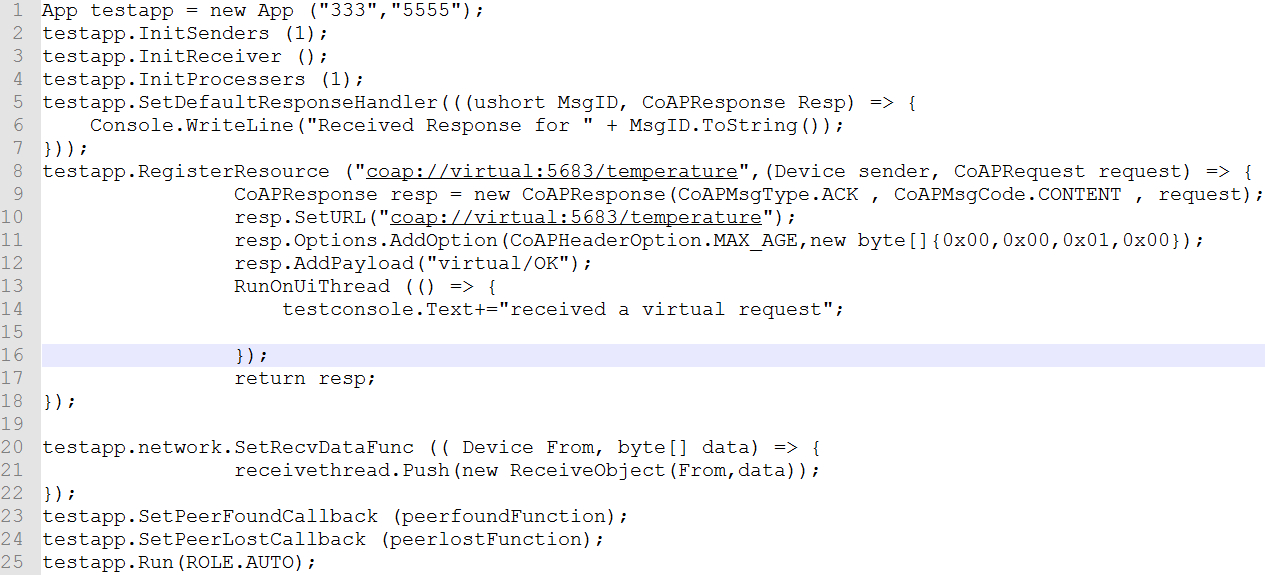
\includegraphics[scale=0.5]{pic/code1.png} 
  \caption{core-code for process componenet}
\end{figure}

As shown below, the communication component of application layer is implemented as an abstract class called "AbstractNetwork". In the abstract class, basic operations of a node have been defined. To support different underlying technologies, the abstract class needs to be inherited by different classes.  

\begin{figure}[H]
  \centering 
      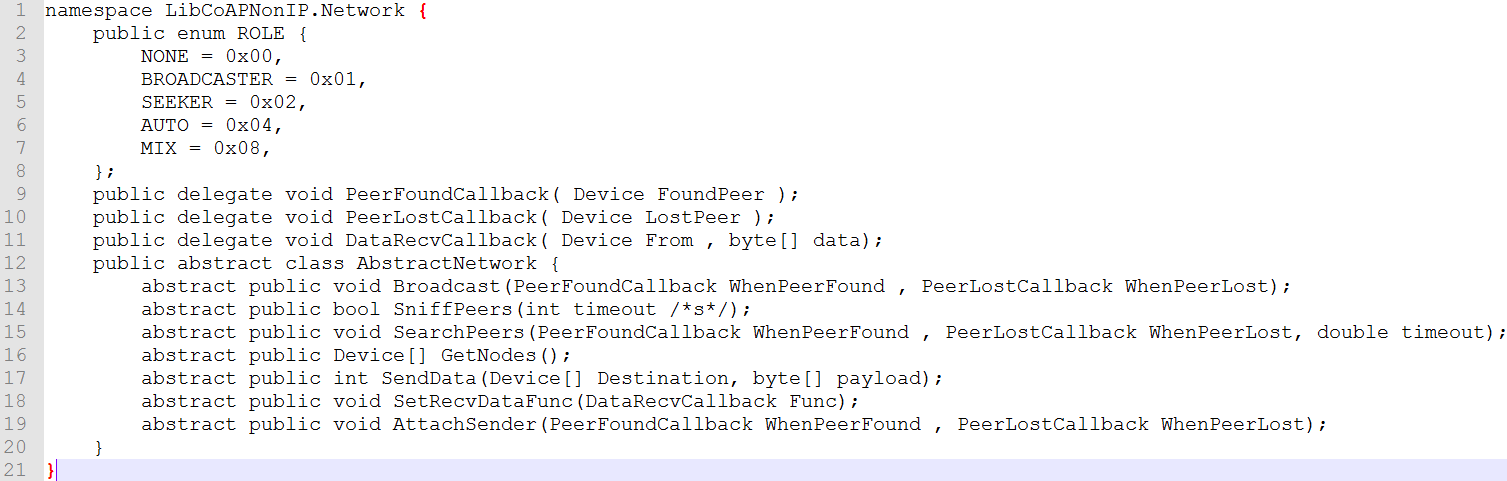
\includegraphics[scale=0.45]{pic/code2.png} 
  \caption{core-code for communication compoennet}
\end{figure}

\section{Network Layer}
In the network layer, two roles need to be supported: Client and Server. Therefore, two kinds of services are defineded. In Android, a component called "Service" is available for customized background running program. The "Service" can get messages from different applications by registering "BroadcastReceiver" and send messages to applications by "Broadcast".

As shown below, both "client service" and "server service" need to register a receiver before scan or broadcast. 

\begin{figure}[h]
  \centering 
      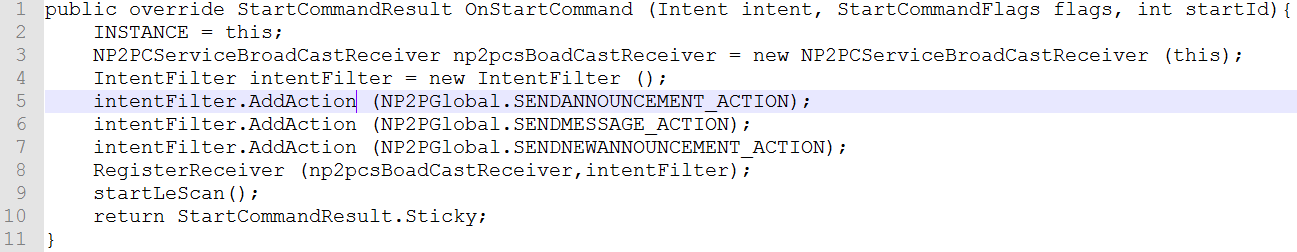
\includegraphics[scale=0.5]{pic/code3.png} 
  \caption{core-code for client service}
\end{figure}
\newpage
\begin{figure}[h]
  \centering 
      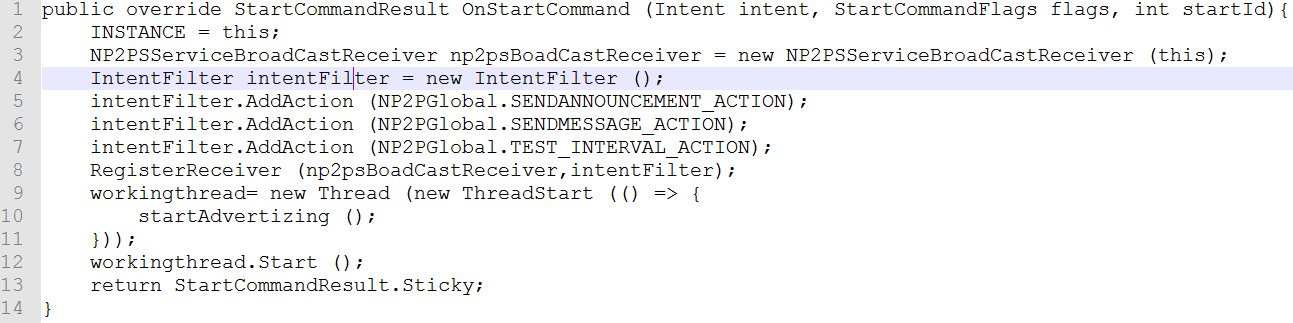
\includegraphics[scale=0.5]{pic/code4.png} 
  \caption{core-code for server service}
\end{figure}

\section{Demo Applicaitons for Experiment}
The procedure of implementation consists of two stages. In the first stage, I implement the BLE infrastructure to send CoAP message. In the second stage, two apps are developed to do the experiments. The first App is called "Major App." It is designed to do first three experiments. The second app is called "Trigger App." It is designed to play the role as a second sender in the fourth experiment ("Multiple Apps").

As shown below, the UI of the "Major App" consists of three sections. The left side contains a list of available devices and a role indicator. The top of the right side is "experiment selection" section with a "start test" button. The remaining section of the right side is the output console where experiment information is recorded. The UI of "Trigger app" is a lite version of that in "Major App" where experiment selection section is disabled. For those experiment apps, the producer threads generate designed packets and call "send request" function to send a message out.

\newpage
\begin{figure}[H]
  \centering 
      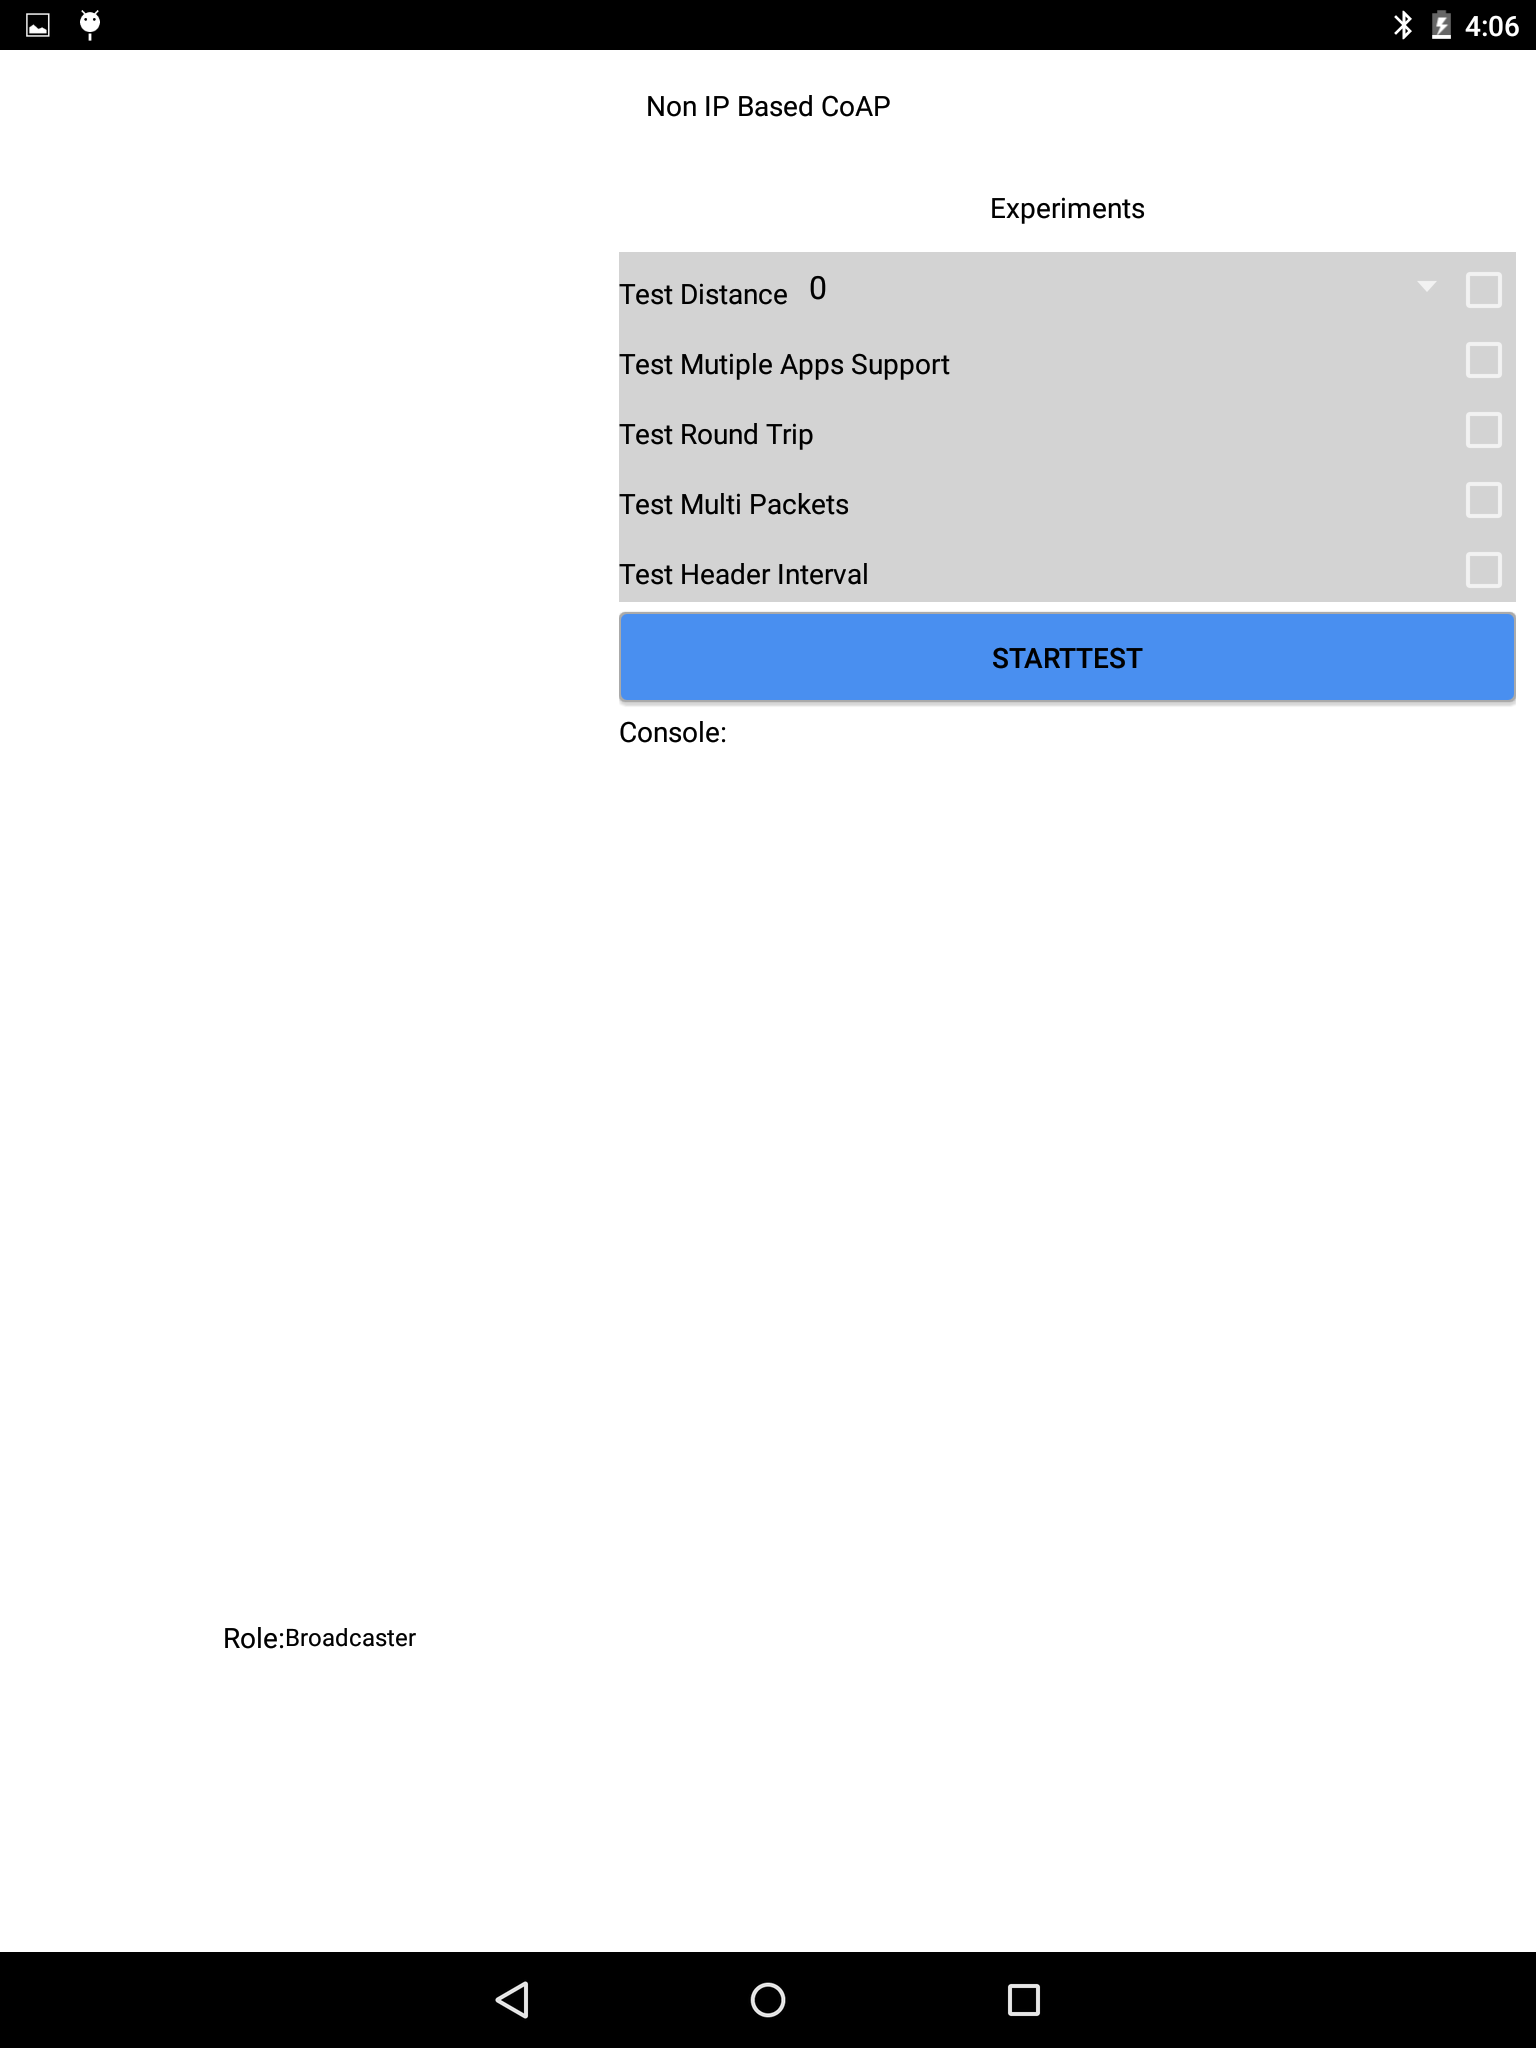
\includegraphics[scale=0.3]{pic/experimentsceenshot.png} 
  \caption{screenshot of demo application}
\end{figure}  

\chapter{Experiments/Evaluations} 
In this chapter, I will evaluate the performance of the proposed architecture in BLE. As mentioned above the architecture is compatible with different technologies. In the implementation, BLE is adopted to make a prototype. So far, all the experiments are under the context of BLE.

Although Bluetooth low energy has been widely tested and adopted, we should keep in mind that Android device to device communication through BLE (peripheral communication) has not been widely tested. So far, only latest Android devices with Bluetooth4.1 hardware support peripheral mode. 
\section{Goals of Experiment}
Five experiments are designed and they are listed in the below table.

\begin{table}[h!]
  \centering
  \caption{Experiment goals}
  \label{tab:table1}
  \begin{tabular}{cc}
    \toprule
    Title & Goals \\
    \midrule
    Minimum Data with Interval & Test performance of sending CoAP header with different intervals. \\
    Multiple Packets & Test performance of sending different CoAP messages with different data size. \\
    Round-Trip & Test performance of round trip \\
    Multiple Apps & Test performance of underlying service to support multiple apps. \\
    \bottomrule
  \end{tabular}
\end{table}
  
\section{Experiment Setup}
As explained earlier, the proposed architecture is designed for server-client communication. Two Android devices are used to do the test. Since only latest hardware with Bluetooth v4.1 supports android to android Bluetooth communication, two Nexus 9 are used to test BLE implementation of the architecture.
\newpage

\begin{table}[h!]
  \centering
  \caption{Experiment goals}
  \label{tab:table1}
  \begin{tabular}{cc}
    \toprule
    Hardware & Details \\
    \midrule
    OS & Android OS, v5.1.1(Lollipop)\\
    CPU & Dual-core 2.3 GHz Denver \\
    Memory & 16GB/2GB RAM \\
    Bluetooth & v4.1, A2DP, apt-X \\
    \bottomrule
  \end{tabular}
\end{table}

Two devices run a test app (more details in implementation chapter). The app can connect two devices together through BLE. 
\section{Details}
In the following sections, I will discuss details of each experiment in "Description", "Procedure" and "Result and Analysis".
\subsection{Minimum Data with Interval}
\subsubsection{Description}
As mentioned in the chapter of design, we implement BLE in sequential-send mode, which means messages are not sent out at the same time. Instead, each message needs to wait for a signal from the remote device before writing a new data to BLE characteristic. In this way, the connection between the devices becomes more stable.

Since the design of BLE aims to support lightweight data transfer, it is important to get its performance with the minimum payload. In this test, I send 4-bytesheader without any payload between two devices. I expect to find some patterns of time cost of sending data with delay. 
\subsubsection{Procedure}

\begin{itemize}
  \item Start sample program scan and create a connection between two devices.
  \item Send 4-byte header (100 times with 0,50,100,150,200,250,300,350,400,450ms respectively) with different intervals to remote devices.
  \item Record received time at sender side (get 99 sets of data). 
  \item Calculate transfer time according to time gap between messages received.
\end{itemize}

\subsubsection{Result and Analysis}

\begin{figure}[H]
  \centering 
      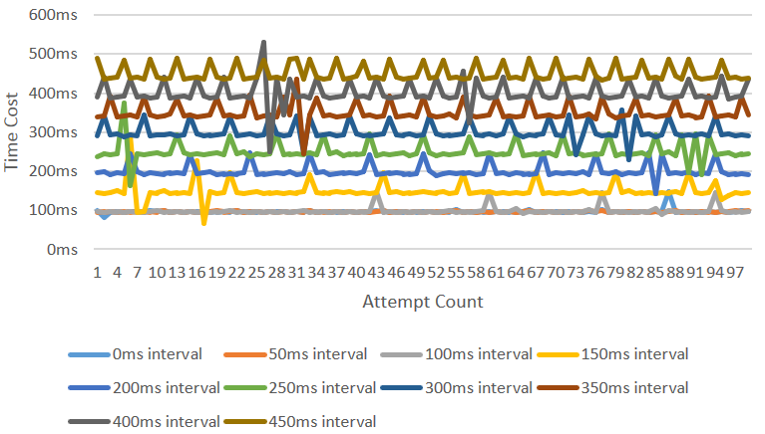
\includegraphics[scale=0.8]{pic/experiment1.png} 
  \caption{Packet structure}
\end{figure}


As shown above, ten series of data were recorded. The x-axis is the number of samples (99 samples for each series). The y-axis is the data transfer time plus waits time (unit is ms). From the above chart, four interesting points were found.
First, the first three series have similar y value. The average time is around 100ms.  Since the sery 4, the Y value increases uniformly by 50ms. The reason is when a message is sent to the message queue with interval 0ms, 50ms, and 100ms, the message does not need to wait before it is sent because the system always needs to wait for a response signal of the previous message before sending a new one out. Since the time of sending a message and waiting for response signal is around 100ms, the message the Y values of first three series are around 100ms.

Second, there is a heartbeat-like pattern in those series. The pattern is always observed with the increasing of intervals. As shown in the blow three charts, the heartbeat-like pattern is also visible with 150ms delay and 200ms delays. The heartbeat-like pattern has similar amplitude (around 50ms). And, the pattern can be explained with energy saving strategy of BLE.

\begin{figure}[H]
  \centering 
      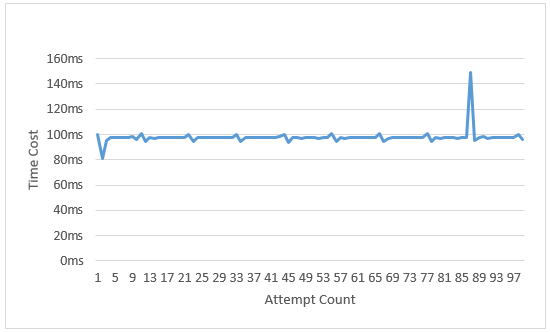
\includegraphics[scale=1]{pic/experiment1result1.png} 
  \caption{Result of sending headers with no interval}
\end{figure}
 
\begin{figure}[H]
  \centering 
      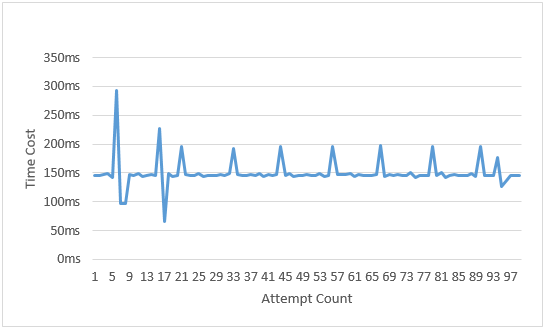
\includegraphics[scale=1]{pic/experiment1result2.png} 
  \caption{Result of sending headers with 150ms interval}
\end{figure}

\begin{figure}[H]
  \centering 
      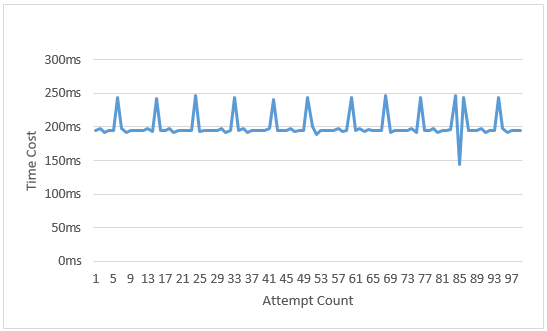
\includegraphics[scale=1]{pic/experiment1result3.png} 
  \caption{Result of sending headers with 200ms interval}
\end{figure}

Third, as shown in the above, there are not only randomly spread fluctuations but also have random amplitudes. This pattern can be explained with a known issue with Android Lollipop’s implementation of BLE.

Last, from those three charts, we know that those random fluctuations become a regular pattern when the system sends data with delay. This phenomenon can be explained by communication interval of BLE.

To further investigate the behaviors of the system, another set of test is designed to focus on the size change of BLE packets.
\subsection{Multiple Packets}
\subsubsection{Description}
From the first experiment, we have found three interesting patterns. The reason for first pattern is obvious. The reasons for the other two to are more complex. Although, I have proposed explanations for the last two patterns, more experiments are needed to verify my assumptions. As explained earlier, we send data in BLE by writing and reading data in BLE characteristic. And, the maximum unit size is 20-byte.
In this experiment, we send multiple BLE packets of data by controlling the payload of the CoAP message. We would like to find out whether the data patterns of one experiment still exist. Meanwhile, we expect more evidence to support our hypothesis of data patterns in the previous experiment.
\subsubsection{Procedure}

\begin{itemize}
  \item Start a sample program scan and create a connection between two devices.
  \item Send CoAP message with 4-byte (1 packet), 12 (2 packets),28 (3 packets), 44 (4 packets), 60(5 packets), 76 (6 packets) and 92(7 packets) bytes payload 100 times respectively (0 interval time).
  \item Record the received time when receiving a response from the connected device. 
  \item Calculate transfer time according to the time gap between messages received.
\end{itemize}

\subsubsection{Result and Analysis}

\begin{figure}[H]
  \centering 
      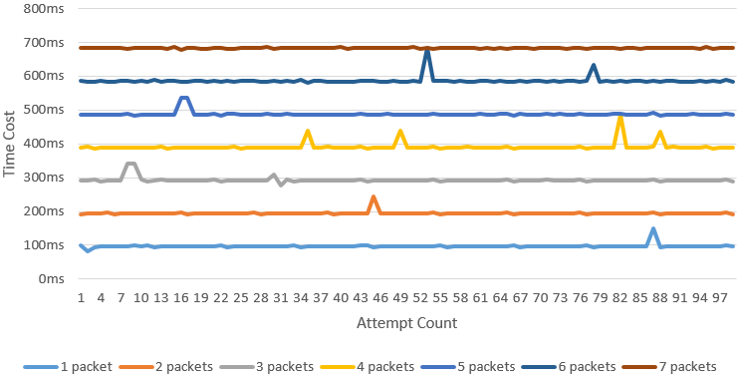
\includegraphics[scale=0.8]{pic/experiment2.png} 
  \caption{Results of sending multiple packets}
\end{figure}

As shown above, the 7 series of data display the performance of the architecture with the increasing size of BLE packets. From the summary chart, we get following information:

\begin{itemize}
  \item With the increasing size of messages, transfer time linearly increases from 100ms to 700ms.
  \item The heartbeat-like pattern still exists.
  \item The random fluctuation observed in previous experiments still exists in the chart.
\end{itemize}

\begin{figure}[H]
  \centering 
      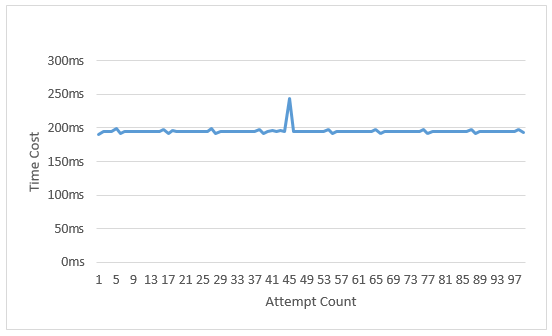
\includegraphics[scale=1]{pic/experiment2result1.png} 
  \caption{Result of sending 12-byte payload}
\end{figure}

\begin{figure}[H]
  \centering 
      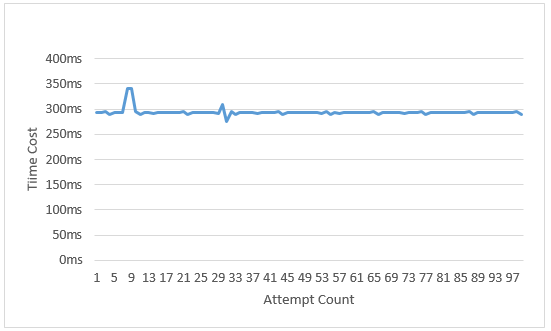
\includegraphics[scale=1]{pic/experiment2result2.png} 
  \caption{Result of sending 28-byte payload}
\end{figure}

As shown above, both random fluctuations and heartbeat-like patterns exist in those two charts. Compared with the detected random fluctuations in experiment one, random fluctuations in the above charts are not predictable. It shows the delay of data will influence the random fluctuation.

This experiment supports our explanation of the random fluctuation and heartbeat-like pattern.
\subsection{Round-Trip}
\subsubsection{Description}
In order to test the performance of real-time data communication between two devices, the round trip experiment is designed, where the receiver of 4-byte header request always sends a response to the sender.
\subsubsection{Procedure}

\begin{itemize}
  \item Start sample program scan and create a connection between two devices.
  \item Send 4-byte header 100 times (0 interval time).
  \item Record received time at sender side (get 99 sets of data).
  \item Calculate round trip time according to the time gap between message received.
  \item Repeat 2 to 4 steps three times.
\end{itemize}

\subsubsection{Result and Analysis} 
\begin{figure}[H]
  \centering 
      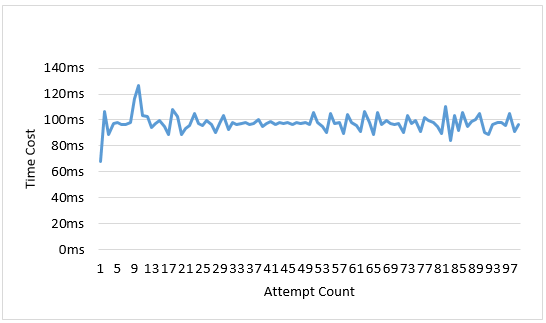
\includegraphics[scale=1]{pic/experiment3result1.png} 
  \caption{First set of 4-byte round trip}
\end{figure}

\begin{figure}[H]
  \centering 
      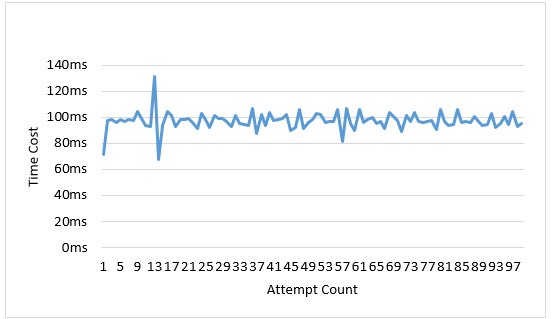
\includegraphics[scale=1]{pic/experiment3result2.png} 
  \caption{Second set of 4-byte round trip}
\end{figure}

\begin{figure}[H]
  \centering 
      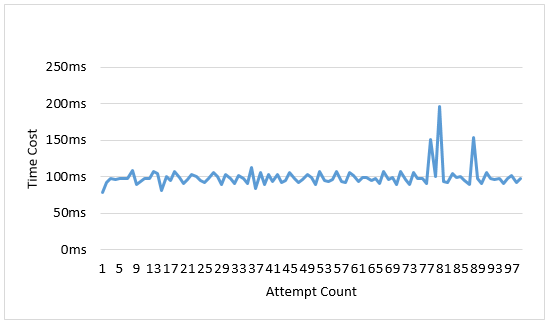
\includegraphics[scale=1]{pic/experiment3result3.png} 
  \caption{Third set of 4-byte round trip}
\end{figure}

In the first experiment, we examined one-way time consumption of 4-byte header CoAP message. The data we got from that experiment shows a pattern obviously. However, according to the charts above, we can not find any pattern for the round trip experiment. Comparing those two experiments, I find that the curve fluctuates greatly around 100ms. Meanwhile, some great fluctuation occurs from time to time. The greater fluctuation of the curve may due to channel interference caused by complex reasons. On the other hand, I believe the random fluctuation here is caused by Android Lollipop’s BLE implementation. 

According to the round trip experiment and the minimum payload experiment, we draw the conclusion that the default communication interval of BLE in Android should be 100ms. Meanwhile, the average time consumption of one-way communication and round trip communication are close in the proposed architecture. 

\subsection{Multiple Apps}
\subsubsection{Description}
The experiment aims to test the performance of underlying network service. In this experiment, the two applications on the same device try to send 100 CoAP headers to the remote device at the same time. The sender side will record total transfer time to calculate average time.
\subsubsection{Procedure}

\begin{itemize}
  \item Start both the "Major APP" and the "Trigger App".
  \item Click start test button at either app to start test.
  \item Record start time and end time at sender side.
  \item Repeat 2-3 steps 10 times.
\end{itemize}

\newpage
\subsubsection{Result and Analysis} 
\begin{figure}[h]
  \centering 
      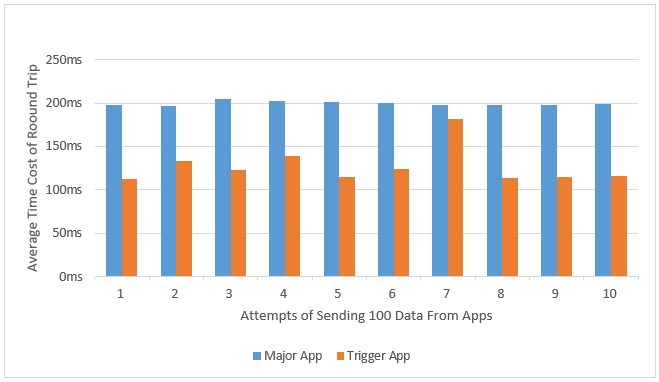
\includegraphics[scale=1]{pic/experiment4.png} 
  \caption{Result of Multi-App Experiment}
\end{figure}

As mentioned above, the two apps use underlying services for CoAP communication. The "Major App" has a listener listening to the event of "start test" from the "Trigger App". After 10 times repeat, there are 10 sets of data available. As shown above, the average time cost of round trip in the "Major App" is always higher than that in "Trigger App". Meanwhile, values of the "Trigger App" are fluctuant. This result is due to the competition of communication channel. Before the "Major App" gets broadcast message, the "Trigger App" can push requests into "send thread" without interruption. Therefore, the "Trigger App" always finishes task earlier.
\section{Conclusion}
Based on the analysis of the experiment results, we have enhanced understanding of implementations of Android’s BLE. Meanwhile, we have obtained more data about the performance of proposed architecture. In previous experiments, we also tested our architecture’s performance in lightweight and medium weight payload communication. According to above analysis, we draw the following conclusions:

\begin{itemize}
  \item The minimum transfer time of proposed architecture is around 100ms. In single communication channel (one characteristic is used to transfer data), we have 16 bytes available to transfer CoAP messages (more details in packet design subchapter). Therefore, in current architecture, the data rate is 10*16 byte/s. 
  \item "Connection interval" is a parameter in BLE. It determines how often a central device exchange data with peripheral. Since the data is specified by device’s implementation, it can be any value between 7.5ms and 4s. It is an important factor to affect data transfer. It is most likely the reason of constant fluctuation when we send data with different latency.
  \item There is a considerable amount of bad performance reports about Android lollipop's implementation of BLE. The Android V5.0 (Lollipop) is the first Android version to support peripheral mode. It is not surprising to get bad performance by the introduction of the new feature. We expect the experimental results can be improved on new Android devices with latest API and BLE hardware. 
  \item Because a single message queue and "send thread" are used to send data in the underlying architecture, the competition of sending messages will influence the send time of a message. 
\end{itemize}

\chapter{Conclusion and Future Work}
\section{Summary and Contributions}
With the development of IoT, more and more small sensors are involved in data collecting. However, different protocols and hardware limitations make communications between devices become more and more difficult. To overcome those limitations, this research proposes an architecture to grant CoAP in BLE. And, it has the potential to support other WPAN technologies as well.

In terms of design and architecture, the proposed architecture consists of two layers. The application layer provides an interface to send and receive CoAP messages as well as the message management. The network layer implements underlying logics of assembling and disassembling CoAP message on the top of Bluetooth Low Energy’s GATT service. The architecture uses two parameters (UserID and AppID) to identify different communication instances. In order to make the architecture works as a background service to serve one or more Apps in one physical device, special packet format and communication principles are designed.

In terms of implementation, Mono is used develop the proposed architecture. Mono is a software platform developed by Xamarin for cross-platform application development in C\#. There are two stages in the implementation. In the first stage, I developed the underlying network layer for Bluetooth Low Energy for Android. In the second stage, developed two test program for the experiments. They are "Major App" and "Trigger App". The "Trigger App" only was used in the last experiment to test the performance of background running service when it serves multiple apps.

In order to test the performance of the proposed architecture, I have done four experiments. Those experiments reveal the cost and limitations of the proposed architecture on the top of BLE’s GATT service.

\begin{itemize}
  \item The first experiment shows that sending a message with interval may have consistent fluctuations.
  \item The second experiment shows that the latency of sending a message increases linearly with the increasing size of BLE packets. 
  \item The third experiment shows that there is no significant time difference between sending one-way and round trip messages in the proposed architecture. Meanwhile, there are random fluctuations. 
  \item The fourth experiment shows that competitions happen when multiple apps try to send messages at the same time.  
\end{itemize}

To achieve four research goals, the architecture adopts various mechanisms:

\begin{itemize}
  \item AppID and UserID are used to identify all devices in a WPAN. This solution unified the way to identify a device.
  \item A "chop" and "assemble" mechanism to overcome the 20-byte size limitation of BLE packet. 
  \item Messages are broadcasted to serve all registered apps.
  \item An interface to abstract operations of communication   
\end{itemize}

In conclusion, the proposed architecture has provided a general solution to achieve cross communication technologies’ CoAP communication in WPAN. So far, although there are some limitations and restrictions to send CoAP messages in BLE, the proposed architecture works on BLE and can serve APPs as a background running service. Since the proposed architecture is capable of supporting different underlying technologies, the low data rate performance should not be a reason to stop explore the potential of the architecture. In order to support other WPAN technologies, more works need to be done in the future.
\section{Future Work}
The proposed architecture can be improved in several aspects. In the following section, I will discuss them in details. 
\subsection{Data Rate}
As shown in the experiments, the average time to send out a CoAP header is around 100ms in the current implementation. According to our analysis, the data rate performance is significantly influenced by the implementation of BLE as well as the sequential data transfer strategy. In the future, data rate could be improved in two ways.  First, latest smart phone with latest Android APIs should be utilized on the architecture. Second, we could explore the possibility to use asynchronous mechanism to send data. 
\subsection{Availability}
In the current version, the network layer does not have cache mechanism. Since the wireless connection is naturally fragile, the cache strategy should be added in the future works. In addition, the reconnection mechanism should also be added.
\subsection{Cross-Platform}
At present, the proposed architecture is implemented in Android because of two facts. First, a developer has the full control of the most hardware. Second, background services are well supported. In the future, attempts should be made to achieve cross-platform implementation in iOS or Windows Phone
\subsection{Underlying Technology}
As mentioned above, the proposed architecture is designed to have the potential to support multiple underlying communication technologies. In the current implementation, it only supports BLE. In further research, the proposed architecture should support more WPAN technologies.
\subsection{Security}
All communications in the current implementation are not encrypted. In further research, the proposed architecture should implement symmetric or asymmetric algorithm encryption to improve its security level.


 
\Urlmuskip=0mu plus 1mu\relax
\uofsbibliography{Nan_Thesis} 
% If you are not using bibtex, comment the line above and uncomment
% the line below.  
%Follow the line below with a thebibliography environmentand bibitems.  
% Note: use of bibtex is usually the preferred method.

%\uofsbibliographynobibtex


%%%%%%%%%%%%%%%%%%%%%%%%%%%%%%%%%%%%%%%%%%%%%%%%%%%%%%%%%%%%%%%%%%%%%%%%%
% APPENDICES
%
% Any chapters appearing after the \appendix command get numbered with
% capital letters starting with appendix 'A'.
% New chapters from here on will be called 'Appendix A', 'Appendix B'
% as opposed to 'Chapter 1', 'Chapter 2', etc.
%%%%%%%%%%%%%%%%%%%%%%%%%%%%%%%%%%%%%%%%%%%%%%%%%%%%%%%%%%%%%%%%%%%%%%%%%%

% Activate thesis appendix mode.
\uofsappendix

\chapter{Link for code}
For more information about detail implementation, Please visit the github link: \url{https://github.com/chennanoka/CoAPNonIP_V1}

%\chapter{Another Sample Appendix}

%Stuff for this appendix goes here.


\end{document}
